\documentclass{book}
\usepackage{graphicx}
\usepackage{tikz}
\usepackage{multirow}
\usepackage{pdfpages}
\usepackage{afterpage}
%\documentclass{article}
\usetikzlibrary{positioning}
\usetikzlibrary{3d} % Para trabajar con proyecciones 3D
%\usetikzlibrary{tikz-3dplot}
%\usepackage[spanish]{babel}
\usetikzlibrary{shapes.misc, arrows, positioning}
\usepackage{float}
\usepackage{amsmath}
\usepackage{enumitem}
\usepackage{tikz-3dplot}
\usepackage{amsmath, amssymb}
\usetikzlibrary{quotes,arrows.meta}
\usepackage{pgfplots}
\usepackage{titlesec}
\usepackage{titlesec}
\usepackage{microtype}
\usetikzlibrary{3d, patterns}
\usepackage{caption}
\usepackage{wrapfig}
\usepackage{tikz-dimline}
\usepackage{verbatim}
\usepackage{empheq}
\renewcommand{\figurename}{Figura}
\pgfplotsset{compat=1.18}


\begin{document}
\part {MEDIOS DE ENLACE}
\title{\LARGE Medios de Enlace: Una guía por el electromagnetismo \\ 
{\small para estudiantes de Ingeniería Electrónica}} 
\author{\small \textbf{Esp. Ing. José Agustín Peralta}} 
\date{} 
\maketitle 
    
\includepdf[pages=1]{mapa_mental.pdf}
\chapter{Algebra Vectorial}

El electromagnetismo es una rama fundamental de la física que estudia la interacción entre las cargas eléctricas y los campos magnéticos. Para describir estas interacciones de forma precisa, necesitamos una matemática que nos permita representar magnitudes físicas con dirección y sentido. Aquí es donde entra en juego el \textbf{álgebra vectorial}. A través de vectores y operaciones vectoriales, podremos expresar conceptos como la fuerza eléctrica, el campo magnético y el flujo magnético de manera concisa y elegante. El álgebra vectorial no solo nos ayudará a comprender las leyes fundamentales del electromagnetismo, sino que también será una herramienta invaluable en el análisis de líneas de transmisión, guías de onda, fibra óptica y antenas. En este módulo, exploraremos los conceptos básicos del álgebra vectorial, sentando las bases para nuestro viaje a través del fascinante mundo del electromagnetismo.

\paragraph{Introducción}

En el mundo que nos rodea, nos encontramos con una gran variedad de magnitudes físicas. Algunas de ellas, como la temperatura de una habitación o la masa de un objeto, se pueden describir completamente con un solo número. Sin embargo, otras magnitudes, como la velocidad del viento o la fuerza que ejerce un imán, requieren que especifiquemos no solo su magnitud, sino también su dirección y sentido. Para representar estas magnitudes de forma precisa, utilizamos \textbf{vectores}. En esta sección, exploraremos la diferencia entre magnitudes escalares y vectoriales, y comprenderemos por qué los vectores son esenciales para el estudio del electromagnetismo.
   
%Revisado

\section{Escalares y Vectores}

En física, una magnitud \textbf{escalar} se define como aquella que queda completamente determinada con un valor numérico y su correspondiente unidad de medición. Un escalar no tiene dirección ni sentido asociado, y se puede operar como un número real (sumar, restar, multiplicar, dividir). Para representar un escalar, se utiliza una letra o un símbolo, sin necesidad de flechas ni negritas. \textbf{Nota:} ésta es la notación que vamos a utilizar a lo largo de esta guía.

Así, por ejemplo, la masa de un electrón es $9.11 \times 10^{-31}$ kg, la temperatura de un conductor es 25 °C, y la carga eléctrica de un protón es $1.602 \times 10^{-19}$ C. Otras magnitudes escalares relevantes en electromagnetismo son la frecuencia de una onda, el potencial eléctrico y la resistencia eléctrica (temas que van a ser tratados en sus respectivos módulos).

\paragraph{Representación en blanco y negro:} Es importante tener en cuenta que, al imprimir esta guía en blanco y negro, la notación para escalares, vectores y dimensiones puede ser diferente. Para los escalares, seguiremos utilizando letras o símbolos sin ningún tipo de marca adicional. Para los vectores, en lugar de usar negritas, utilizaremos una flecha sobre la letra. Las dimensiones y las unidades se representarán entre corchetes, como $[L]$ para longitud, $[M]$ para masa y $[T]$ para tiempo.

\section{Magnitud y dirección de Vectores: El vector unitario y componentes de un vector}

A diferencia de las magnitudes escalares, que quedan definidas con un número y una unidad, las magnitudes vectoriales requieren que especifiquemos su magnitud, dirección y sentido. Para representar un vector gráficamente, utilizamos el sistema de coordenadas cartesianas. En él dibujamos el vector mediante una flecha, donde la longitud de la flecha representa la magnitud y la punta de la flecha indica la dirección y el sentido. La dirección de un vector se refiere a la línea recta a lo largo de la cual actúa el vector, y el sentido indica hacia qué lado de la línea apunta el vector. Ejemplos de magnitudes vectoriales en física son: la velocidad, la aceleración y la fuerza. En electromagnetismo, trabajaremos con vectores como el campo eléctrico, el campo magnético y el momento dipolar para enunciar algunos de los vectores que vamos a utilizar.

Para describir la dirección de un vector en un sistema de coordenadas cartesianas, utilizamos vectores unitarios. Un vector unitario es un vector \textbf{de magnitud 1} que apunta en una dirección específica. En tres dimensiones, los vectores unitarios se denotan como \textbf{$\hat{a}_x$},  \textbf{$\hat{a}_y$} y \textbf{$\hat{a}_z$}, y apuntan en la dirección de los ejes $x, y, z$ respectivamente.

Cualquier vector en tres dimensiones se puede expresar como una combinación lineal de los vectores unitarios. Los coeficientes de esta combinación lineal se denominan componentes escalares del vector. Por ejemplo, un vector $\mathbf{A}$ se puede escribir como:

\begin{equation}
\mathbf{A} = A_x \hat{a}_x + A_y \hat{a}_y + A_z \hat{a}_z
\label{eq:vector_componentes}
\end{equation}

donde $A_x$, $A_y$ y $A_z$ son las componentes escalares del vector $\mathbf{A}$ en las direcciones $x, y, z$ respectivamente.

\begin{figure}[h!]
    \centering
    \tdplotsetmaincoords{60}{130}

    \begin{tikzpicture}[tdplot_main_coords]
        \draw[thick,->] (0,0,0) -- (3,0,0) node[anchor=north east]{$x$};
        \draw[thick,->] (0,0,0) -- (0,3,0) node[anchor=north west]{$y$};
        \draw[thick,->] (0,0,0) -- (0,0,3) node[anchor=south]{$z$};

        \draw[ultra thick,->,blue] (0,0,0) -- (1.5,2,2) node[anchor=south west]{$\mathbf{A}$}; % Nuevas coordenadas
        \draw[thick,->,red] (0,0,0) -- (1,0,0) node[anchor=north west]{$\mathbf{a_x}$};
        \draw[thick,->,red] (0,0,0) -- (0,1,0) node[anchor=north east]{$\mathbf{a_y}$};
        \draw[thick,->,red] (0,0,0) -- (0,0,1) node[anchor=south east]{$\mathbf{a_z}$};
        \node[anchor=north] at (1.5,0,0) {$A_x$};
        \node[anchor=east] at (0,2,0) {$A_y$};
        \node[anchor=west] at (0,0,2) {$A_z$};

        % Proyecciones
        \draw[thin, dashed, red] (1.5,2,2) -- (1.5,2,0);
        \draw[thin, dashed, red] (1.5,2,0) -- (0,2,0);
        \draw[thin, dashed, red] (1.5,2,0) -- (1.5,0,0);

        \draw[thin, dashed, green] (1.5,2,2) -- (1.5,0,2);
        \draw[thin, dashed, green] (1.5,0,2) -- (1.5,0,0);
        \draw[thin, dashed, green] (1.5,0,2) -- (0,0,2);

        \draw[thin, dashed, purple] (1.5,2,2) -- (0,2,2);
        \draw[thin, dashed, purple] (0,2,2) -- (0,2,0);
        \draw[thin, dashed, purple] (0,2,2) -- (0,0,2);
    \end{tikzpicture}
    \caption{Vector A en 3 dimensiones y sus componentes escalares.}
    \label{fig:vector_componentes}
\end{figure}

En esta guía, seguiremos las siguientes convenciones para la notación de variables:

\begin{itemize}
    \item[\textbullet] \textbf{Variables vectoriales:} Se representarán con letras en \textbf{negrita}, como $\mathbf{E}$ para el campo eléctrico, o con una flecha sobre la letra, como $\vec{E}$, cuando sea necesario para evitar confusiones.
    \item[\textbullet] \textbf{Variables escalares:} Se representarán con letras mayúsculas o minúsculas sin negrita, como $Q$ para la carga eléctrica o $V$ para el potencial eléctrico.
    \item[\textbullet] \textbf{Dimensiones o Unidades:} Se indicarán entre corchetes, como $[L]$ para longitud, $[M]$ para masa y $[T]$ para tiempo.
\end{itemize}
Además, antes de utilizar una variable en una ecuación importante o en la resolución de problemas, la declararemos explícitamente, indicando su tipo y su significado. Por ejemplo:

\begin{itemize}
    \item[\textbullet] $Q$: escalar, carga eléctrica de la partícula.
    \item[\textbullet] $\mathbf{E}$: vector, campo eléctrico.
    \item[\textbullet] $[T]$: dimensión, tiempo.
\end{itemize}

Esta práctica ayudará a evitar confusiones y a que el lector comprenda claramente el significado de cada variable, especialmente al imprimir la guía en blanco y negro o realizar copias de la misma. Esta notación también será la que se utilizará en el desarrollo de los ejercicios en clase.

\section{Suma y Resta de Vectores}

Para trabajar en electromagnetismo es fundamental que recordemos algunos conceptos sobre el álgebra vectorial que estudiamos en materias anteriores como Álgebra y Geometría Analítica. Entre esos conceptos que necesitamos recordar están la suma y resta de vectores. Al igual que con los números, podemos realizar operaciones de suma y resta con vectores. Sin embargo, debido a que los vectores tienen magnitud y dirección, estas operaciones tienen características especiales que debemos tener en cuenta cuando vamos a realizarlas.

\subsection{Suma de vectores:}

\begin{itemize}
    \item \textbf{Método gráfico:} Para sumar dos vectores $\mathbf{A}$ y $\mathbf{B}$ gráficamente, podemos utilizar el método del paralelogramo.
    \item \textbf{Método del paralelogramo:} Se dibujan los vectores $\mathbf{A}$ y $\mathbf{B}$ con su origen en el mismo punto. Luego, se construye un paralelogramo con $\mathbf{A}$ y $\mathbf{B}$ como lados adyacentes. La diagonal del paralelogramo que parte del origen común de $\mathbf{A}$ y $\mathbf{B}$ representa la suma $\mathbf{A} + \mathbf{B}$.
    \item \textbf{Método analítico:} Para sumar vectores analíticamente, se suman las componentes correspondientes de cada vector. Si $\mathbf{A} = (A_x, A_y, A_z)$ y $\mathbf{B} = (B_x, B_y, B_z)$, entonces $\mathbf{A} + \mathbf{B} = (A_x + B_x, A_y + B_y, A_z + B_z)$.
\end{itemize}

\begin{figure}[h!]
    \centering
    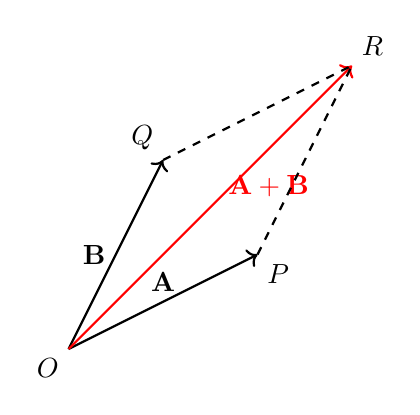
\begin{tikzpicture}[scale=1.2]
    \draw[thick,->] (0,0) -- (2,1) node[midway, above] {$\mathbf{A}$}; % Vector A
    \draw[thick,->] (0,0) -- (1,2) node[midway, left] {$\mathbf{B}$}; % Vector B
    \draw[thick,->,red] (0,0) -- (3,3) node[midway, above right, xshift=1mm] {$\mathbf{A} + \mathbf{B}$}; % Vector A + B
    \draw[thick,dashed] (2,1) -- (3,3); % Lado del paralelogramo
    \draw[thick,dashed] (1,2) -- (3,3); % Lado del paralelogramo
    % Etiquetas para los vértices
    \node[below left] at (0,0) {$O$};
    \node[below right] at (2,1) {$P$};
    \node[above left] at (1,2) {$Q$};
    \node[above right] at (3,3) {$R$};
    \end{tikzpicture}
    \caption{Suma de vectores mediante el método del paralelogramo.}
    \label{fig:paralelogramo}
\end{figure}

\subsection{Resta de vectores:}

\begin{itemize}
    \item \textbf{Definición:} La resta de dos vectores $\mathbf{A}$ y $\mathbf{B}$ se define como la suma del vector $\mathbf{A}$ con el opuesto del vector $\mathbf{B}$, es decir, $\mathbf{A} - \mathbf{B} = \mathbf{A} + (-\mathbf{B})$.
    \item \textbf{Método gráfico:} Para restar dos vectores $\mathbf{A}$ y $\mathbf{B}$ gráficamente, se dibuja el vector $\mathbf{A}$ y el vector $-\mathbf{B}$ (que tiene la misma magnitud que $\mathbf{B}$ pero sentido opuesto). Luego, se suman los vectores $\mathbf{A}$ y $-\mathbf{B}$ utilizando el método del paralelogramo.
    \item \textbf{Método analítico:} Para restar vectores analíticamente, se restan las componentes correspondientes de cada vector. Si $\mathbf{A} = (A_x, A_y, A_z)$ y $\mathbf{B} = (B_x, B_y, B_z)$, entonces $\mathbf{A} - \mathbf{B} = (A_x - B_x, A_y - B_y, A_z - B_z)$.
\end{itemize}

\subsection{Propiedades de la suma y resta de vectores:}

\begin{itemize}
    \item \textbf{Conmutatividad:} La suma de vectores es conmutativa: $\mathbf{A} + \mathbf{B} = \mathbf{B} + \mathbf{A}$.
    \item \textbf{Asociatividad:} La suma de vectores es asociativa: $(\mathbf{A} + \mathbf{B}) + \mathbf{C} = \mathbf{A} + (\mathbf{B} + \mathbf{C})$.
    \item \textbf{Existencia del vector cero:} Existe un vector cero, denotado como $\mathbf{0}$, que cumple que $\mathbf{A} + \mathbf{0} = \mathbf{A}$ para cualquier vector $\mathbf{A}$.
    \item \textbf{Existencia del vector opuesto:} Para cada vector $\mathbf{A}$ existe un vector opuesto $-\mathbf{A}$, tal que $\mathbf{A} + (-\mathbf{A}) = \mathbf{0}$.
\end{itemize}

\subsection{Aplicaciones:} 

La suma y resta de vectores tienen numerosas aplicaciones en física e ingeniería, como el cálculo de fuerzas resultantes, velocidades resultantes, análisis de circuitos eléctricos (fasores), etc.


%Revisado 

\section{Multiplicación de un vector por un escalar}

\paragraph{Introducción:}

En el álgebra vectorial, no solo podemos sumar y restar vectores, sino que también podemos multiplicarlos por escalares (números reales). Esta operación, aunque sencilla en apariencia, tiene un gran impacto en la forma en que representamos y manipulamos magnitudes físicas. Imaginemos, por ejemplo, que queremos duplicar la fuerza que se aplica sobre un objeto, o que necesitamos invertir el sentido del campo eléctrico en una región del espacio. ¿Cómo podemos lograr esto? La respuesta está en la multiplicación de un vector por un escalar.

Esta operación nos da un "control" similar al que tenemos con los filtros de Instagram. Así como podemos aumentar el brillo o la saturación de una foto, al multiplicar un vector por un escalar podemos modificar su magnitud y dirección, creando nuevas posibilidades para describir el mundo que nos rodea.

\subsection{Definición:}

Al multiplicar un vector $\mathbf{A}$ por un escalar $k$, se obtiene un nuevo vector $k\mathbf{A}$ cuya magnitud es $|k|$ veces la magnitud de $\mathbf{A}$, y cuya dirección es la misma que la de $\mathbf{A}$ si $k$ es positivo, o la opuesta si $k$ es negativo.

\begin{figure}[H]
\centering
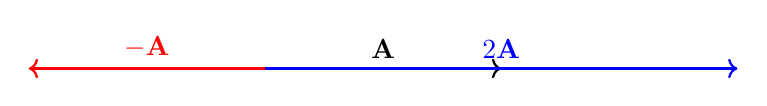
\begin{tikzpicture}[scale=1.5]

\draw[thick,->] (0,0) -- (2,0) node[midway, above] {$\mathbf{A}$}; % Vector A
 \draw[thick,->,blue] (0,0) -- (4,0) node[midway, above] {$2\mathbf{A}$}; % Vector 2A
 \draw[thick,->,red] (0,0) -- (-2,0) node[midway, above] {$-\mathbf{A}$}; % Vector -A

\end{tikzpicture}
\caption{Multiplicación del vector $\mathbf{A}$ por los escalares 2 y -1.}
\label{fig:multiplicacion_escalar}
\end{figure}

\paragraph{Ejemplo:}

Si $\mathbf{A}$ es un vector de magnitud 3 unidades que apunta hacia la derecha, y $k = 2$, entonces $2\mathbf{A}$ será un vector de magnitud 6 unidades que también apunta hacia la derecha. Si $k = -1$, entonces $-\mathbf{A}$ será un vector de magnitud 3 unidades que apunta hacia la izquierda.

\paragraph{En resumen:}

\begin{itemize}
\item[\textbullet] La multiplicación por un escalar positivo estira o comprime el vector, manteniendo su dirección.
\item[\textbullet] La multiplicación por un escalar negativo estira o comprime el vector e invierte su dirección.
\end{itemize}

\subsection{Propiedades de la multiplicación por un escalar:}

La multiplicación de un vector por un escalar cumple con las siguientes propiedades:

\begin{itemize}
\item[\textbullet] \textbf{Distributiva respecto a la suma de vectores:} $k (\mathbf{A} + \mathbf{B}) = k\mathbf{A} + k\mathbf{B}$
 \item[\textbullet] \textbf{Distributiva respecto a la suma de escalares:} $(k + l)\mathbf{A} = k\mathbf{A} + l\mathbf{A}$
\item[\textbullet] \textbf{Asociativa:} $(k l)\mathbf{A} = k(l\mathbf{A})$
\item[\textbullet] \textbf{Multiplicación por 1:} $1\mathbf{A} = \mathbf{A}$
\end{itemize}

Estas propiedades son similares a las propiedades de la multiplicación de números reales, y nos permiten manipular expresiones con vectores y escalares de forma flexible.

\section{Producto de vectores}

\paragraph{Introducción:}

Además de la suma, la resta y la multiplicación por un escalar, existen otras operaciones que podemos realizar con vectores. En particular, el producto escalar y el producto vectorial son dos operaciones que combinan dos vectores para producir un nuevo objeto (un escalar o un vector, respectivamente).

\subsection{Producto escalar o producto punto}

\subsubsection{Definición:} 

El producto escalar de dos vectores $\mathbf{A}$ y $\mathbf{B}$, denotado por $\mathbf{A} \cdot \mathbf{B}$, se define como el producto de sus magnitudes y el coseno del ángulo más pequeño entre ellos:

\begin{empheq}[box=\fbox]{align*}
\mathbf{A} \cdot \mathbf{B} &\equiv |\mathbf{A}||\mathbf{B}| \cos \theta
\end{empheq}

donde $|\mathbf{A}|$ y $|\mathbf{B}|$ son las magnitudes de los vectores $\mathbf{A}$ y $\mathbf{B}$ respectivamente, y $\theta$ es el ángulo entre ellos.

\subsubsection{Interpretación geométrica:} 

El producto escalar se puede interpretar geométricamente como el producto de la magnitud de la proyección de $\mathbf{A}$ sobre $\mathbf{B}$ por la magnitud de $\mathbf{B}$.

\begin{equation}
\mathbf{A} \cdot \mathbf{B} = (A \cos \theta) |\mathbf{B}| = |\mathbf{A}| (B \cos \theta)
\label{eq:producto_punto}
\end{equation}

\begin{figure}[H]
\centering
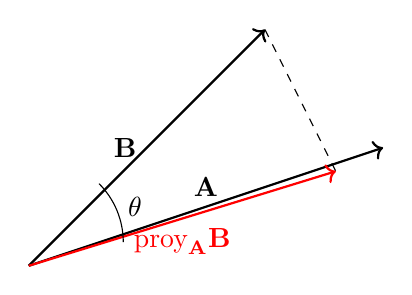
\begin{tikzpicture}[scale=1.5]

 \draw[thick,->] (0,0) -- (3,1) node[midway, above] {$\mathbf{A}$}; % Vector A
\draw[thick,->] (0,0) -- (2,2) node[midway, left] {$\mathbf{B}$}; % Vector B

 \draw[dashed] (2,2) -- (2.6,0.8); % Línea de proyección
 \draw[thick,->,red] (0,0) -- (2.6,0.8) node[midway, below] {$\text{proy}_{\mathbf{A}} \mathbf{B}$}; % Proyección de B sobre A

 % Ángulo entre los vectores
 \draw[thin] (0.8,0.2) arc (0:45:0.7); % Coordenadas modificadas
 \node at (0.9,0.5) {$\theta$}; % Coordenadas modificadas

\end{tikzpicture}
\caption{Proyección del vector $\mathbf{B}$ sobre el vector $\mathbf{A}$.}
\label{fig:proyeccion_vectorial_B_sobre_A}
\end{figure}

\subsubsection{Propiedades}

El producto escalar tiene las siguientes propiedades:

\begin{itemize}
 \item[\textbullet] \textbf{Conmutatividad:} $\mathbf{A} \cdot \mathbf{B} = \mathbf{B} \cdot \mathbf{A}$
\item[\textbullet] \textbf{Distributividad:} $\mathbf{A} \cdot (\mathbf{B} + \mathbf{C}) = \mathbf{A} \cdot \mathbf{B} + \mathbf{A} \cdot \mathbf{C}$
 \item[\textbullet] \textbf{Asociatividad con un escalar:} $(k\mathbf{A}) \cdot \mathbf{B} = k(\mathbf{A} \cdot \mathbf{B}) = \mathbf{A} \cdot (k\mathbf{B})$
 \item[\textbullet] \textbf{Producto de un vector por sí mismo:} $\mathbf{A} \cdot \mathbf{A} = |\mathbf{A}|^2$
\end{itemize}

\subsubsection{Expresión en coordenadas cartesianas:} 

Si $\mathbf{A} = (A_x, A_y, A_z)$ y $\mathbf{B} = (B_x, B_y, B_z)$, entonces:

\begin{equation}
\mathbf{A} \cdot \mathbf{B} = A_xB_x + A_yB_y + A_zB_z
\label{eq:producto_punto_cartesianas}
\end{equation}

\subsubsection{Aplicaciones:} 

El producto escalar tiene numerosas aplicaciones en física e ingeniería, tales como:

\begin{itemize}
 \item[\textbullet] Calcular el trabajo realizado por una fuerza.
 \item[\textbullet] Determinar el ángulo entre dos vectores.
 \item[\textbullet] Calcular la componente de un vector en una dirección dada.
 \item[\textbullet] Verificar si dos vectores son ortogonales (perpendiculares).
\end{itemize}


\subsection{Producto Vectorial o Producto Cruz}

\subsubsection{Definición:} 

El producto vectorial de dos vectores $\mathbf{A}$ y $\mathbf{B}$, denotado por $\mathbf{A} \times \mathbf{B}$, es un nuevo vector $\mathbf{C}$ cuya definición es: \textit{“el vector cuya magnitud es el valor absoluto del producto de las magnitudes de los dos vectores por el seno del ángulo menor entre los dos vectores, mientras que la dirección del vector es perpendicular al plano en el que se encuentran los dos vectores”}.

\begin{empheq}[box=\fbox]{align*}
|\mathbf{C}| = |\mathbf{A} \times \mathbf{B}| &\equiv |\mathbf{A}| |\mathbf{B}| \sin \theta
\end{empheq}

\begin{itemize}
 \item[\textbullet] \textbf{Magnitud:} La magnitud de $\mathbf{C}$ es igual al producto de las magnitudes de $\mathbf{A}$ y $\mathbf{B}$ por el seno del ángulo $\theta$ entre ellos.
 \item[\textbullet] \textbf{Dirección:} $\mathbf{C}$ es perpendicular al plano que contiene a los vectores $\mathbf{A}$ y $\mathbf{B}$.
 \item[\textbullet] \textbf{Sentido:} El sentido de $\mathbf{C}$ se determina por la regla de la mano derecha: Si se coloca la mano derecha de manera que los dedos apunten en la dirección del vector $\mathbf{A}$ y se curvan hacia el vector $\mathbf{B}$ a través del ángulo $\theta$, entonces el pulgar apuntará en la dirección de $\mathbf{C}$. El ángulo $\theta$ es el menor de los ángulos que se pueden formar entre ambos vectores.
 \end{itemize}
\subsubsection{Interpretación geométrica:} La magnitud del producto vectorial $|\mathbf{A} \times \mathbf{B}|$ es igual al área del paralelogramo formado por los vectores $\mathbf{A}$ y $\mathbf{B}$.


\subsubsection{Propiedades:} 

El producto vectorial tiene las siguientes propiedades:

\begin{itemize}
\item[\textbullet] \textbf{Anticonmutatividad:} $\mathbf{A} \times \mathbf{B} = - (\mathbf{B} \times \mathbf{A})$
 \item[\textbullet] \textbf{Distributividad:} $\mathbf{A} \times (\mathbf{B} + \mathbf{C}) = \mathbf{A} \times \mathbf{B} + \mathbf{A} \times \mathbf{C}$
 \item[\textbullet] \textbf{Asociatividad con un escalar:} $(k \mathbf{A}) \times \mathbf{B} = k (\mathbf{A} \times \mathbf{B}) = \mathbf{A} \times (k \mathbf{B})$
 \item[\textbullet] \textbf{Producto vectorial por sí mismo:} $\mathbf{A} \times \mathbf{A} = \mathbf{0}$
\end{itemize}

\subsubsection{Expresión en coordenadas cartesianas:} 

Si $\mathbf{A} = (A_x, A_y, A_z)$ y $\mathbf{B} = (B_x, B_y, B_z)$, entonces el producto vectorial $\mathbf{A} \times \mathbf{B}$ se puede calcular mediante el siguiente determinante:

\begin{equation}
\mathbf{A} \times \mathbf{B} =
\begin{vmatrix}
\mathbf{\hat{a}_x} & \mathbf{\hat{a}_y} & \mathbf{\hat{a}_z} \\
A_x & A_y & A_z \\
B_x & B_y & B_z
\end{vmatrix}
\label{eq:producto_cruz_cartesiano}
\end{equation}

donde $\mathbf{\hat{a}_x}$, $\mathbf{\hat{a}_y}$ y $\mathbf{\hat{a}_z}$ son los vectores unitarios en las direcciones $x$, $y$ y $z$ respectivamente.

\subsubsection{Aplicaciones:} 

El producto vectorial tiene numerosas aplicaciones en física e ingeniería, tales como:

\begin{itemize}
 \item[\textbullet] Calcular el momento de una fuerza.
 \item[\textbullet] Calcular el flujo magnético a través de una superficie.
 \item[\textbullet] Describir la fuerza magnética sobre una carga en movimiento.
\end{itemize}

\begin{figure}[H]
\centering
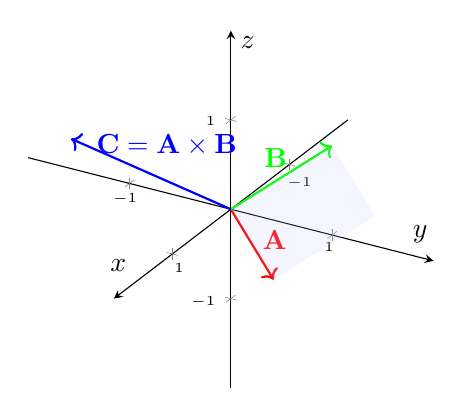
\begin{tikzpicture}
\begin{axis}[
 view={120}{30}, % Ajusta la vista 3D
 axis lines=center,
 xlabel={$x$},
 ylabel={$y$},
 zlabel={$z$},
 xmin=-2, xmax=2,
 ymin=-2, ymax=2,
 zmin=-2, zmax=2,
 xtick={-1,0,1},
 ytick={-1,0,1},
 ztick={-1,0,1}, % Ajusta las marcas de los ejes
 xticklabel style={font=\tiny},
 yticklabel style={font=\tiny},
 zticklabel style={font=\tiny},
 width=0.8\textwidth, % Ancho de la figura
 height=0.8\textwidth, % Altura de la figura (ajustada proporcionalmente)
]

% Define los vectores A y B
\coordinate (A) at (1,1,0);
\coordinate (B) at (0,1,1);

% Dibuja los vectores A y B
\draw[thick,->,red] (axis cs:0,0,0) -- (axis cs:1,1,0) node[midway, above right, yshift=-2mm] {$\mathbf{A}$};
\draw[thick,->,green] (axis cs:0,0,0) -- (axis cs:0,1,1) node[midway, above left, xshift=2mm] {$\mathbf{B}$};

% Calcula el producto vectorial C = A x B
\coordinate (C) at (1,-1,1);

% Dibuja el vector C
\draw[thick,->,blue] (axis cs:0,0,0) -- (axis cs:1,-1,1) node[midway, above, xshift=2mm, yshift=1mm] {$\mathbf{C} = \mathbf{A} \times \mathbf{B}$};

% Dibuja el plano formado por A y B con sombreado
\fill[opacity=0.2, blue!20] (axis cs:0,0,0) -- (axis cs:1,1,0) -- (axis cs:1,2,1) -- (axis cs:0,1,1) -- cycle;

\end{axis}
\end{tikzpicture}
\caption{Producto vectorial de dos vectores $\mathbf{A}$ y $\mathbf{B}$. El vector resultante $\mathbf{C}$ es perpendicular al plano formado por $\mathbf{A}$ y $\mathbf{B}$.}
\label{fig:producto_vectorial_sin_proyecciones}
\end{figure}

%Revisado I

\section{Definición de campos}

\subsection{Introducción:}

Un campo es una región del espacio donde se define una magnitud física en cada punto. Esta magnitud puede ser escalar o vectorial, lo que da lugar a dos tipos de campos: campos escalares y campos vectoriales.

Esta idea es similar a la de las funciones de varias variables que estudiaron en Análisis Matemático II. Así como una función $f(x, y, z)$ asigna un valor a cada punto $(x, y, z)$ en el espacio, un campo también asigna una magnitud (escalar o vectorial) a cada punto.

\subsection{Campos escalares:}

Un campo escalar es aquel en el que a cada punto del espacio se le asigna un valor numérico (un escalar). Podemos representarlo matemáticamente como una función escalar de tres variables: $f(x, y, z)$ donde $f$ es el valor del campo escalar en el punto $(x, y, z)$.

\subsubsection{Ejemplos:}
\begin{itemize}
    \item [\textbullet]Temperatura en una habitación: $T(x, y, z)$
    \item [\textbullet]Presión atmosférica: $P(x, y, z)$
    \item [\textbullet]Potencial eléctrico: $V(x, y, z)$
    \item [\textbullet]Densidad de carga: $\rho(x, y, z)$
\end{itemize}

\subsection{Campos vectoriales:}

Un campo vectorial es aquel en el que a cada punto del espacio se le asigna un vector. Podemos representarlo matemáticamente como una función vectorial:

$\mathbf{F}(x, y, z) = F_x(x, y, z) \mathbf{\hat{a}}_x + F_y(x, y, z) \mathbf{\hat{a}}_y + F_z(x, y, z) \mathbf{\hat{a}}_z$ donde $\mathbf{F}$ es el vector del campo en el punto $(x, y, z)$, y $F_x$, $F_y$, $F_z$ son sus componentes escalares en las direcciones de los vectores unitarios $\mathbf{\hat{a}}_x$, $\mathbf{\hat{a}}_y$ y $\mathbf{\hat{a}}_z$.

\subsubsection{Ejemplos:}
\begin{itemize}
    \item [\textbullet]Campo gravitatorio: $\mathbf{g}(x, y, z)$
    \item [\textbullet]Campo eléctrico: $\mathbf{E}(x, y, z)$
    \item [\textbullet]Campo magnético: $\mathbf{H}(x, y, z)$ (o $\mathbf{B}(x, y, z)$)
    \item [\textbullet]Velocidad del viento: $\mathbf{v}(x, y, z)$
\end{itemize}

\begin{figure} [h!]
    \centering
    \includegraphics[scale=0.5]{Algebra Vectorial/campo_vectorial1.pdf}
    \caption{Ejemplo de un campo Vectorial con Python}
    \label{fig: campo_vectorial1}
\end{figure}
\subsection{Representación gráfica de campos escalares}

\begin{figure} [h!]
    \centering
    \includegraphics[scale=0.5]{Algebra Vectorial/campo_vectorial2.pdf}
    \caption{Ejemplo Campo Vectorial con Python}
    \label{fig:campo_vectorial2}
\end{figure}

\subsubsection{Introducción:}

Para visualizar un campo escalar, utilizamos mapas de isolíneas o curvas de nivel. Estas son curvas que conectan puntos con el mismo valor del campo. Imagina un mapa topográfico, donde las curvas de nivel representan puntos con la misma altitud. De manera similar, en un mapa de isolíneas de un campo escalar, las curvas conectan puntos con el mismo valor del campo.

  
\subsubsection{Construcción de un mapa de isolíneas:}


Para construir un mapa de isolíneas, seguimos estos pasos:

\begin{enumerate}
\item Elegimos un conjunto de valores representativos del campo escalar.
\item Para cada valor, identificamos los puntos en el espacio que tienen ese valor.
\item Unimos esos puntos mediante curvas suaves, que son las isolíneas.
\end{enumerate}

\subsubsection{Características de las isolíneas:}

Las isolíneas tienen características importantes que nos ayudan a interpretar el campo escalar:

\begin{itemize}
\item[\textbullet] Las isolíneas nunca se cruzan entre sí, ya que un punto en el espacio no puede tener dos valores diferentes del campo escalar.
\item[\textbullet] La densidad de las isolíneas indica la magnitud del gradiente del campo escalar: cuanto más juntas estén las isolíneas, mayor es el gradiente (o variación) del campo en esa región. \textbf{Nota:}Veremos el concepto de gradiente en detalle en el próximo módulo.
\item[\textbullet] Las isolíneas cerradas indican máximos o mínimos locales del campo escalar.
\end{itemize}

\subsubsection{Ejemplos:}

Veamos algunos ejemplos de campos escalares y sus mapas de isolíneas:

\begin{itemize}
\item[\textbullet] \textbf{Temperatura en una habitación:} Las isolíneas conectarían puntos con la misma temperatura. Podríamos observar zonas más calientes y zonas más frías en la habitación.
\item[\textbullet] \textbf{Presión atmosférica:} En un mapa meteorológico, las isolíneas de presión (isobaras) conectan puntos con la misma presión atmosférica. Estas líneas nos ayudan a identificar zonas de alta y baja presión, que están relacionadas con los fenómenos climáticos.
\item[\textbullet] \textbf{Potencial eléctrico:} Las isolíneas de potencial eléctrico (equipotenciales) conectan puntos con el mismo potencial. Estas líneas nos ayudan a visualizar la distribución del potencial eléctrico en una región con cargas.
\end{itemize}

\subsubsection{Herramientas para la visualización:}

Para crear mapas de isolíneas, podemos utilizar diferentes herramientas:

\begin{itemize}
\item[\textbullet] \textbf{Lenguajes de programación:} Phyton, MATLAB.
\item[\textbullet] \textbf{Software de graficación:} Tikz.
\item[\textbullet] \textbf{Herramientas online:} Existen varias herramientas online que permiten crear mapas de isolíneas de forma interactiva.
\end{itemize}
\begin{figure} [h!]
    \centering
    \includegraphics[scale=0.5]{campo_escalarpy}
    \caption{Campo escalar sinusoidal}
    \label{fig:campo_escalar}
\end{figure}


\begin{figure} [h!]
    \centering
    \includegraphics[scale=0.5]{Algebra Vectorial/mapa_isolineas.pdf}
    \caption{Ejemplo de Mapa de isolíneas}
    \label{mapa_isolineas}
\end{figure}

\newpage
\section{Sistemas de coordenadas}

\subsection{Introducción:}

En el estudio del electromagnetismo, es fundamental poder describir la posición de cargas, corrientes y campos en el espacio. Para ello, utilizamos sistemas de coordenadas, que son conjuntos de reglas que nos permiten especificar la ubicación de un punto. En esta sección, estudiaremos los tres sistemas de coordenadas más utilizados en electromagnetismo: cartesiano, cilíndrico y esférico.

Una característica importante de estos sistemas es que son \textbf{ortogonales}: los vectores unitarios que definen las direcciones de los ejes son perpendiculares entre sí en cada punto del espacio. Esto significa que, al representar un punto en cualquiera de estos sistemas, lo hacemos en referencia a vectores unitarios que forman ángulos rectos entre sí. 

Es importante destacar que, aunque algunos vectores unitarios representan desplazamientos lineales (como $\mathbf{\hat{a}}_x$, $\mathbf{\hat{a}}_y$, $\mathbf{\hat{a}}_z$ en coordenadas cartesianas o  $\mathbf{\hat{a}}_\rho$ en coordenadas cilíndricas) y otros representan desplazamientos angulares (como $\mathbf{\hat{a}}_\phi$ en coordenadas cilíndricas o $\mathbf{\hat{a}}_\theta$ y $\mathbf{\hat{a}}_\phi$ en coordenadas esféricas), la ortogonalidad se mantiene. Los vectores unitarios, ya sean lineales o angulares, siempre son perpendiculares entre sí en cada punto del espacio.

La ortogonalidad de los sistemas de coordenadas facilita la descripción de fenómenos físicos y la resolución de problemas en electromagnetismo. Por ejemplo, al calcular la fuerza entre dos cargas, podemos descomponerla en sus componentes a lo largo de los ejes ortogonales, lo que simplifica el análisis.

\subsection{Sistema de coordenadas cartesianas:}

El sistema cartesiano es el más familiar. Utiliza tres ejes perpendiculares entre sí, que se suelen denotar como $x$, $y$ y $z$. La posición de un punto se define mediante sus coordenadas $(x, y, z)$, que representan las distancias del punto a cada uno de los planos formados por los otros dos ejes.

Los vectores unitarios en este sistema se denotan como $\mathbf{\hat{a}}_x$, $\mathbf{\hat{a}}_y$ y $\mathbf{\hat{a}}_z$, y apuntan en la dirección positiva de los ejes $x$, $y$ y $z$ respectivamente.

Las coordenadas cartesianas son especialmente útiles en problemas donde la geometría se alinea con los ejes cartesianos, como el cálculo del campo eléctrico o del potencial eléctrico debido a la distribución de cargas puntuales o lineales a lo largo de un alambre finito cargado.
 
 \begin{figure}[H]
     \centering
     \tdplotsetmaincoords{70}{110}
     \begin{tikzpicture}[tdplot_main_coords,scale=1.1]
  \draw[thick,->] (0,0,0) -- (4,0,0) node[anchor=north east]{$x$};
  \draw[thick,->] (0,0,0) -- (0,4,0) node[anchor=north west]{$y$};
  \draw[thick,->] (0,0,0) -- (0,0,4) node[anchor=south]{$z$};

  \draw[thick,->,red] (0,0,0) -- (1,0,0) node[anchor=north west]{$\mathbf{\hat{a}}_x$};
  \draw[thick,->,red] (0,0,0) -- (0,1,0) node[anchor=north east]{$\mathbf{\hat{a}}_y$};
  \draw[thick,->,red] (0,0,0) -- (0,0,1) node[anchor=south east, yshift=-3mm]{$\mathbf{\hat{a}}_z$};

  % Proyecciones como caja en líneas de trazos
  \draw[dashed] (2,0,0) -- (2,2,0) -- (0,2,0);
  \draw[dashed] (2,2,0) -- (2,2,2) -- (0,2,2) -- (0,0,2);
  \draw[dashed] (0,0,2) -- (2,0,2) -- (2,2,2);
  \draw[dashed] (2,0,0) -- (2,0,2);
  \draw[dashed] (0,2,0) -- (0,2,2);
  \node[anchor=south west, above] at (2,2,2){\textcolor{blue}{P(x,y,z)}};
  \node[anchor=north, above left] at (2,0,0) {$x$};
  \node[anchor=east, above left] at (0,2,0) {$y$};
  \node[anchor=west, above right] at (0,0,2) {$z$};
\end{tikzpicture}
     \caption{Punto en un sistema de Coordenadas Cartesianas}
     \label{fig:enter-label}
 \end{figure}
%\tdplotsetmaincoords{70}{110}  % Nuevos ángulos de visión

\subsubsection{Diferencial de longitud $dl$}

En coordenadas cartesianas, el diferencial de longitud $dl$ representa un pequeño segmento de línea recta en el espacio. Se puede expresar como la suma vectorial de sus componentes en las direcciones de los ejes $x$, $y$ y $z$:

\[
    dl = dx \mathbf{\hat{a}}_x + dy \mathbf{\hat{a}}_y + dz \mathbf{\hat{a}}_z
\]

donde $dx$, $dy$ y $dz$ son las longitudes de las proyecciones de $dl$ sobre los ejes $x$, $y$ y $z$, respectivamente.

\begin{figure}[H]
     \centering
\tdplotsetmaincoords{70}{110}  % Nuevos ángulos de visión
\begin{tikzpicture}[tdplot_main_coords, scale=1.1]
  \draw[thick,->] (0,0,0) -- (4,0,0) node[anchor=north east]{$x$};
  \draw[thick,->] (0,0,0) -- (0,4,0) node[anchor=north west]{$y$};
  \draw[thick,->] (0,0,0) -- (0,0,4) node[anchor=south]{$z$};

  \draw[thick,->,blue] (2,2,2) -- (4,4,4) node[midway,above]{$dl$}; 
% vectores unitarios
 \draw[thick,->,red] (0,0,0) -- (1,0,0) node[anchor=north west]{$\mathbf{\hat{a}}_x$};
  \draw[thick,->,red] (0,0,0) -- (0,1,0) node[anchor=north east]{$\mathbf{\hat{a}}_y$};
  \draw[thick,->,red] (0,0,0) -- (0,0,1) node[anchor=south east, yshift=-3mm]{$\mathbf{\hat{a}}_z$};
  % Proyecciones como caja en líneas de trazos
  \draw[dashed] (2,0,0) -- (2,2,0) node[anchor=east, above, midway, yshift=-4mm]{$dy$} -- (0,2,0);
  \draw[dashed] (2,2,0) -- (2,2,2) --  (0,2,2) node[anchor=north, above left, midway, xshift=-2cm]{$dx$} -- (0,0,2);
  \draw[dashed] (0,0,2) -- (2,0,2) -- (2,2,2);
  \draw[dashed] (2,0,0) -- (2,0,2);
  \draw[dashed] (0,2,0) -- (0,2,2) node[anchor=west, above right, midway, xshift=-3.5cm]{$dz$};
  %Ejes trasladados en el punto
  \draw[thick, ->] (2,2,2)--(2,2,2.5) node[anchor=north, above right, xshift=-4mm, yshift=-1mm]{{$\mathbf{\hat{a}}_z$}$dz$};
  \draw[thick, ->] (2,2,2)--(2.5,2,2) node[anchor=north west, above left,yshift=-2mm, xshift=1mm ]{{$\mathbf{\hat{a}}_x$}$dx$};
  \draw[thick, ->] (2,2,2)--(2,2.5,2)node[anchor=north east, below right, xshift=-4mm, yshift=1mm]{{$\mathbf{\hat{a}}_y$}$dy$};
  \end{tikzpicture}
 \caption{Diferencial de longitud}
     \label{fig:enter-label}
 \end{figure}

La magnitud del diferencial de longitud $dl$ se calcula mediante el teorema de Pitágoras:
\[
|dl| = \sqrt{dx^2 + dy^2 + dz^2}
\]
\subsubsection{Aplicaciones del diferencial de longitud}

El diferencial de longitud $dl$ se utiliza en diversas aplicaciones en electromagnetismo, como:

\begin{itemize}
\item[\textbullet] Calcular el trabajo realizado por una fuerza a lo largo de una trayectoria.
\item[\textbullet] Calcular la circulación de un campo vectorial a lo largo de una curva cerrada.
\item[\textbullet] Calcular el flujo de un campo vectorial a través de una superficie.
\end{itemize}

\subsubsection{Elemento de volumen}

El diferencial de longitud también se utiliza para definir el elemento de volumen $dV$ en coordenadas cartesianas. El elemento de volumen es un pequeño cuboide con lados $dx$, $dy$ y $dz$: $dV = dx dy dz$

\begin{figure}[H]
     \centering
\tdplotsetmaincoords{70}{110} 
\begin{tikzpicture}[tdplot_main_coords, scale=1.2]
  \draw[thick,->] (0,0,0) -- (4,0,0) node[anchor=north east]{$x$};
  \draw[thick,->] (0,0,0) -- (0,4,0) node[anchor=north west]{$y$};
  \draw[thick,->] (0,0,0) -- (0,0,4) node[anchor=south]{$z$};

  % Proyecciones como caja en líneas de trazos (despegada del origen)
  \draw[dashed] (1.5,1,0.5) -- (2.5,1,0.5) -- (2.5,2,0.5) -- (1.5,2,0.5) -- cycle;
  \draw[dashed] (2.5,1,0.5) -- (2.5,1,1.5) -- (2.5,2,1.5) -- (2.5,2,0.5);
  \draw[dashed] (1.5,2,0.5) -- (1.5,2,1.5) -- (2.5,2,1.5);
  \draw[dashed] (1.5,1,1.5) -- (2.5,1,1.5);
  \draw[dashed] (1.5,1,1.5) -- (1.5,2,1.5);
  \draw[dashed] (1.5,1,0.5) -- (1.5,1,1.5);

  % Proyección en el plano xz
  \draw[thin, dashed] (1.5,0,0.5) -- (2.5,0,0.5) node[anchor=north east , above, midway, xshift=3mm]{$dx$} -- (2.5,0,1.5) node[anchor=north west, above left, midway]{$dz$} -- (1.5,0,1.5) -- cycle; 

  % Proyección en el plano yz
  \draw[thin, dashed] (0,1,0.5) -- (0,2,0.5) node[anchor=north west , above, midway, xshift=1mm, yshift=-1mm]{$dy$}  -- (0,2,1.5) node[anchor=south, above right, midway]{$dz$} -- (0,1,1.5) -- cycle; 

% Cotas sobre los ejes
  \draw[thick,<->,red] (1.5,0,0) -- (2.5,0,0) node[midway, below, xshift=2mm, yshift=2mm]{$dx$};
  \draw[thick,<->,red] (0,1,0) -- (0,2,0) node[midway,left, xshift=3mm, yshift=-3mm]{$dy$};
  \draw[thick,<->,red] (0,0,0.5) -- (0,0,1.5) node[midway, right, xshift=-1mm]{$dz$};
 
  % Proyección en el plano xy
  \draw[thin, dashed] (1.5,1,0)  -- (2.5,1,0)node[anchor=north east , above, midway, xshift=-1mm, yshift=-1mm]{$dx$} -- (2.5,2,0) -- (1.5,2,0) node[anchor=north west , above left, midway]{$dy$} -- cycle; 

  % Etiquetas de las proyecciones
  \end{tikzpicture}
\caption{Elemento de Volumen}
     \label{fig:cuboide}
 \end{figure}
 
\subsubsection{Diferenciales de superficie y su orientación}

En electromagnetismo, a menudo es necesario evaluar funciones vectoriales sobre superficies, lo que implica realizar integraciones de superficie. Para esto, es fundamental definir la \textbf{orientación de la superficie}, la cual se establece a través de un vector normal. Este vector normal tiene una magnitud igual al diferencial de superficie y se expresa en coordenadas cartesianas como:
\begin{equation}
dS_x = dy\,dz, \quad dS_y = dx\,dz, \quad dS_z = dx\,dy
\end{equation}
Cada uno de estos elementos vectoriales está dirigido en la dirección del vector unitario normal a la superficie correspondiente.

Para garantizar resultados coherentes, definimos un \textbf{vector de superficie positivo} como aquel que apunta hacia el exterior del volumen delimitado por la superficie. En el caso de una superficie cerrada, la dirección positiva se identifica fácilmente, como se observa en la Figura~\ref{fig:orientacion_superficies}(a). Sin embargo, en superficies abiertas, es necesario decidir qué lado se considerará el "exterior" y cuál el "interior". Esto puede ser ambiguo, como se muestra en la Figura~\ref{fig:orientacion_superficies}(b), donde no es evidente cuál de las dos direcciones es positiva.

Para resolver esta ambigüedad, recurrimos a la \textbf{regla de la mano derecha}. Si los dedos de la mano derecha siguen la dirección en que recorremos el contorno de la superficie abierta, con la palma apuntando hacia el interior, entonces el pulgar señala la dirección positiva de la normal. Esto se ilustra en la Figura~\ref{fig:orientacion_superficies}(c). Cabe destacar que la dirección positiva puede cambiar si invertimos el sentido del recorrido en el contorno.

En términos prácticos, la elección de la dirección positiva depende del contexto físico, como la ubicación de fuentes o la dirección en la que se realizarán los cálculos. Por ejemplo, en un sistema donde la superficie no está cerrada, es común definir la dirección positiva como aquella que apunta hacia afuera de las fuentes.

Finalmente, un elemento de superficie como \( dS_z = dx\,dy \) debe entenderse como el producto de un escalar, que representa el diferencial de superficie, y el vector unitario normal \( \mathbf{\hat{z}} \). Este vector normal puede ser positivo o negativo dependiendo de la orientación establecida, como se observa en las figuras.

\textbf{Nota:} Los elementos de superficie definidos anteriormente no representan componentes vectoriales de un área, sino que describen la dirección normal y el diferencial de superficie. Por lo tanto, cada elemento debe considerarse un vector independiente.


\begin{figure} [H]
    \centering
    \tdplotsetmaincoords{60}{110}

\begin{tikzpicture}[scale=2,tdplot_main_coords]

% Define the radius of the circle
\def\radius{1}

% --- First circle (left) ---
\begin{scope}[shift={(-3,0,0)}]
    \draw[thick, fill=gray!20] (0,0,0) circle (\radius);
    \draw[->, color=red, line width=1.5pt] (0,0,0) -- (0,0,1) node[midway, right] {$\mathbf{\hat{n}}$};
    \node at (0, -1.5, 0) {(a)};
    % Arrows on the perimeter
    \draw[->,>=stealth, line width=1pt] (0,0,0) ++(\radius,0) arc (0:90:\radius);
    \draw[->,>=stealth, line width=1pt] (0,0,0) ++(0,\radius) arc (90:180:\radius);
    \draw[->,>=stealth, line width=1pt] (0,0,0) ++(-\radius,0) arc (180:270:\radius);
    \draw[->,>=stealth, line width=1pt] (0,0,0) ++(0,-\radius) arc (270:360:\radius);

    % Grid on the circle (Adjusted for 3D perspective)
    \foreach \i in {-4,-3,...,4}{
        \draw[thin, gray] (0,0,0) ++({0.2*\i*\radius},{-sqrt(1-0.04*\i*\i)*\radius},0) -- ++({0},{2*sqrt(1-0.04*\i*\i)*\radius},0);
        \draw[thin, gray] (0,0,0) ++({-sqrt(1-0.04*\i*\i)*\radius},{0.2*\i*\radius},0) -- ++({2*sqrt(1-0.04*\i*\i)*\radius},{0},0);
    }

\end{scope}

% --- Second circle (middle) ---
\begin{scope}[shift={(0,0,0)}]
    \draw[thick, fill=gray!20] (0,0,0) circle (\radius);
    \draw[->, color=red, line width=1.5pt] (0,0,0) -- (0,0,1) node[midway, right] {$\mathbf{\hat{n}}$};
    \draw[->, color=red, line width=1.5pt, dashed] (0,0,0) -- (0,0,-1) node[midway, right] {$\mathbf{\hat{n}}$?};
    \node at (0, -1.5, 0) {(b)};
    % Arrows on the perimeter
    \draw[->,>=stealth, line width=1pt] (0,0,0) ++(\radius,0) arc (0:90:\radius);
    \draw[->,>=stealth, line width=1pt] (0,0,0) ++(0,\radius) arc (90:180:\radius);
    \draw[->,>=stealth, line width=1pt] (0,0,0) ++(-\radius,0) arc (180:270:\radius);
    \draw[->,>=stealth, line width=1pt] (0,0,0) ++(0,-\radius) arc (270:360:\radius);
\end{scope}

% --- Third circle (right) ---
\begin{scope}[shift={(3,0,0)}]
    \draw[thick, fill=gray!20] (0,0,0) circle (\radius);
    \draw[->, color=red, line width=1.5pt] (0,0,0) -- (0,0,1) node[midway, right] {$\mathbf{\hat{n}}$};
    \node at (0, -1.5, 0) {(c)};
    % Arrows on the perimeter
    \draw[->,>=stealth, line width=1pt] (0,0,0) ++(\radius,0) arc (0:90:\radius);
    \draw[->,>=stealth, line width=1pt] (0,0,0) ++(0,\radius) arc (90:180:\radius);
    \draw[->,>=stealth, line width=1pt] (0,0,0) ++(-\radius,0) arc (180:270:\radius);
    \draw[->,>=stealth, line width=1pt] (0,0,0) ++(0,-\radius) arc (270:360:\radius);
\end{scope}

% Draw the x, y, and z axes
\draw[->] (0,0,0) -- (4,0,0) node[anchor=north east]{$x$};
\draw[->] (0,0,0) -- (0,2,0) node[anchor=north west]{$y$};
\draw[->] (0,0,0) -- (0,0,1.5) node[anchor=south]{$z$};

\end{tikzpicture}

    \caption{Dirección de una superficie. a) Superficie de una sola cara. b) Superficie c)Regla de la mano derecha}
    \label{fig:orientacion_superficies}
\end{figure}

\begin{figure}[h!]
    \centering
   \tdplotsetmaincoords{60}{110}

\begin{tikzpicture}[scale=3,tdplot_main_coords]

% --- Cubo en perspectiva ---
\begin{scope}[shift={(1,2,2)}]
    % Define the side length of the cube
    \def\side{1}

    % Draw the cube
    % Bottom face (hidden)
    \draw[thick, dashed] (0,0,0) -- (\side,0,0) -- (\side,\side,0) -- (0,\side,0);
    \draw[thick, dashed] (0,0,0) -- (0,\side, 0);
    % Top face (visible)
    \draw[thick] (0,0,\side) -- (\side,0,\side) -- (\side,\side,\side) -- (0,\side,\side) -- cycle;
    % Vertical edges (some hidden)
    \draw[thick, dashed] (0,0,0) -- (0,0,\side);
    \draw[thick] (\side,0,0) -- (\side,\side,0);
    \draw[thick] (\side,0,0) -- (\side,0,\side);
    \draw[thick] (0,\side,0) -- (\side,\side,0);
    \draw[thick] (\side,\side,0) -- (\side,\side,\side);
    \draw[thick] (0,\side,0) -- (0,\side,\side);

    % Dimension lines (Cotas)
    \draw[<->,>=stealth, dashed] (0,-0.2,\side) -- node[fill=white, midway, font=\scriptsize] {$dx$} (\side,-0.2,\side);
    \draw[<->,>=stealth, dashed] (\side,-0.2,0) -- node[fill=white, midway, font=\scriptsize] {$dz$} (\side,-0.2,\side);
    \draw[<->,>=stealth, dashed] (\side+0.2,0,0) -- node[fill=white, midway, font=\scriptsize, sloped] {$dy$} (\side+0.2,\side,0);

    % Unit vector on the top face
    \draw[->, color=red, line width=1.5pt] (\side/2,\side/2,\side) -- (\side/2,\side/2,\side+0.5) node[midway, right, yshift=-3mm] {$\mathbf{\hat{z}}dxdy$};
    \draw[color=black] (\side/2,\side/2,\side) node[scale=0.7]{$+$}; % Cruz

    % Unit vector on the bottom face (dashed)
    \draw[->, color=red, line width=1.5pt, dashed] (\side/2,\side/2,0) -- (\side/2,\side/2,-0.5) node[midway, left, yshift=3mm] {$\mathbf{\hat{-z}}dxdy$};
    \draw[color=black] (\side/2,\side/2,0) node[scale=0.7]{$+$}; % Cruz

    % Unit vector on the right face
    \draw[->, color=blue, line width=1.5pt] (\side,\side/2,\side/2) -- (\side+0.5,\side/2,\side/2) node[midway, below, xshift=5mm, yshift=2mm] {$\mathbf{\hat{x}}dydz$};
    \draw[color=black] (\side,\side/2,\side/2) node[scale=0.7]{$+$}; % Cruz

    % Unit vector on the left face (dashed)
    \draw[->, color=blue, line width=1.5pt, dashed] (0,\side/2,\side/2) -- (-0.5,\side/2,\side/2) node[midway, above, xshift=-6mm, yshift=-2mm ] {$\mathbf{\hat{-x}}dydz$};
    \draw[color=black] (0,\side/2,\side/2) node[scale=0.7]{$+$}; % Cruz

    % Unit vector on the front face
    \draw[->, color=green, line width=1.5pt] (\side/2,\side/2+0.5,\side/2) -- (\side/2,\side+0.5,\side/2) node[midway, right, xshift=2mm, yshift=2mm] {$\mathbf{\hat{y}}dxdz$};
    \draw[color=black] (\side/2,\side/2+0.5,\side/2) node[scale=0.7]{$+$}; % Cruz

    % Unit vector on the back face (dashed)
    \draw[->, color=green, line width=1.5pt, dashed] (\side/2,0,\side/2) -- (\side/2,-0.5,\side/2) node[midway, right, xshift=-1mm, yshift=2mm] {$\mathbf{\hat{-y}}dxdz$};
    \draw[color=black] (\side/2,0,\side/2) node[scale=0.7]{$+$}; % Cruz
\end{scope}

% --- Ejes coordenados en la esquina inferior izquierda ---
\begin{scope}[shift={(-1.5,-1.5,0)}, scale=0.3]
    \draw[->,>=stealth] (0,0,0) -- (1.5,0,0) node[anchor=north east]{$x$};
    \draw[->,>=stealth] (0,0,0) -- (0,1.5,0) node[anchor=north west]{$y$};
    \draw[->,>=stealth] (0,0,0) -- (0,0,1.5) node[anchor=south]{$z$};
\end{scope}
\end{tikzpicture}
    \caption{Dirección de los elementos de superficie en un cubo}
    \label{fig:diferencial_volumen_cartesiana}
\end{figure}
\subsubsection{Diferencial de volumen en coordenadas cartesianas}

El \textbf{diferencial de volumen} $dV$ es un elemento fundamental en el cálculo vectorial aplicado al electromagnetismo, ya que permite integrar funciones tridimensionales, como la densidad de carga eléctrica $\rho$ o la densidad de corriente $\mathbf{J}$. En coordenadas cartesianas, este elemento se define como:
\begin{equation}
dV = dx\,dy\,dz
\end{equation}

En la Figura~\ref{fig:diferencial_volumen_cartesiana}, se ilustra un diferencial de volumen como un pequeño paralelepípedo alineado con los ejes cartesianos. Cada cara del paralelepípedo corresponde a un elemento de superficie con su respectiva normal, lo cual facilita la comprensión de los diferenciales de superficie en el contexto de integraciones volumétricas.

Para analizar este volumen diferencial, se proyectan sus caras en los planos coordenados:
\begin{itemize}
    \item En el \textbf{plano $xy$}, el área proyectada es $dx\,dy$, con una normal orientada en la dirección positiva o negativa del eje $z$.
    \item En el \textbf{plano $xz$}, el área proyectada es $dx\,dz$, con normal en la dirección positiva o negativa del eje $y$.
    \item En el \textbf{plano $yz$}, el área proyectada es $dy\,dz$, con normal en la dirección positiva o negativa del eje $x$.
\end{itemize}

El diferencial de volumen $dV$ se utiliza en integrales del tipo:
\begin{equation}
Q = \iiint_V \rho\,dV
\end{equation}
donde $Q$ representa la carga total contenida en el volumen $V$, y $\rho$ es la densidad de carga volumétrica.

\textbf{Importancia práctica:} Este concepto es esencial para describir fenómenos electromagnéticos, como el flujo de campo eléctrico o magnético, y se aplica tanto en superficies cerradas como en volúmenes abiertos. La proyección de áreas en los planos coordenados, junto con la identificación de las normales asociadas, es clave para desarrollar una intuición sólida sobre las integrales de volumen.

\textbf{Nota:} La orientación de las normales juega un papel importante en aplicaciones como la ley de Gauss o el cálculo de flujos mediante el teorema de divergencia.

\subsection{Sistemas de Coordenadas cilíndricas}

\subsubsection{Introducción al sistema de coordenadas cilíndricas}

El \textbf{sistema de coordenadas cilíndricas} es una extensión del sistema de coordenadas polares en el plano, añadiendo un eje vertical ($z$) para describir puntos en el espacio tridimensional. Este sistema es especialmente útil para resolver problemas con \textit{simetría cilíndrica}, como los campos eléctricos y magnéticos generados por conductores rectos, cilindros o solenoides.

En coordenadas cilíndricas, la posición de un punto $P$ en el espacio se define mediante tres parámetros:
\begin{itemize}
    \item $r$: la distancia perpendicular desde el punto al eje $z$ (radio).
    \item $\phi$: el ángulo que forma la proyección del punto sobre el plano $xy$ con respecto al eje $x$ (ángulo azimutal).
    \item $z$: la altura del punto sobre el plano $xy$.
\end{itemize}

La relación entre las coordenadas cilíndricas $(r, \phi, z)$ y las coordenadas cartesianas $(x, y, z)$ es:
\begin{align}
x &= r \cos\phi, \\
y &= r \sin\phi, \\
z &= z.
\end{align}

\begin{figure} [!h]
    \centering
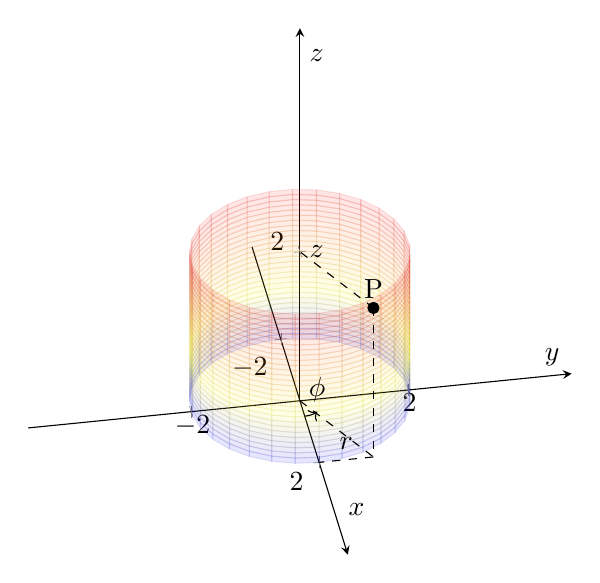
\begin{tikzpicture}[scale=1]
\begin{axis}[
    view={80}{40}, % Ajusta la vista 3D
    axis lines=center,
    xlabel=$x$,
    ylabel=$y$,
    zlabel=$z$,
    xmin=-5, xmax=5,
    ymin=-5, ymax=5,
    zmin=0, zmax=5,
    xtick={-2,0,2}, 
    ytick={-2,0,2}, 
    ztick={2}, % Ajusta las marcas de los ejes
    width=0.8\textwidth,  % Ancho de la figura
    height=0.9\textwidth, % Altura de la figura (ajustada proporcionalmente)
]
% Dibuja el cilindro
\addplot3[surf, opacity=0.1, domain=0:360, y domain=0:2, samples=30] 
    ({2*cos(x)}, {2*sin(x)}, {y});

% Dibuja el punto P y sus coordenadas
\addplot3[mark=*, only marks] coordinates {(2,1,2)};
\node[anchor=south west, above] at (axis cs:2,1,2) {P}; 

% Proyecciones del punto P
\draw[dashed] (axis cs:2,1,2) -- (axis cs:2,1,0);
\draw[dashed] (axis cs:2,1,0) -- (axis cs:2,0,0);
\draw[dashed] (axis cs:0,0,0) -- (axis cs:2,1,0);
\draw[dashed] (axis cs:2,1,2) -- (axis cs:0,0,2);
\draw[->] (axis cs:0.5,0,0) arc (0:45:0.35) node[above] {$\phi$};
% Etiquetas de las coordenadas
\node[above] at (axis cs:2,0.5,0) {$r$};
%\node[anchor=west] at (axis cs:2,1,0) {$\phi$};
\node[anchor=west] at (axis cs:0,0,2) {$z$};
\end{axis}
\end{tikzpicture}
   \caption{Punto P en Coordenadas Cilíndricas}
    \label{fig:coordenadas_cilindricas}
\end{figure}
Por otro lado, la conversión de cartesianas a cilíndricas se realiza mediante:
\begin{align}
r &= \sqrt{x^2 + y^2}, \\
\phi &= \tan^{-1}\left(\frac{y}{x}\right), \\
z &= z.
\end{align}



En la Figura~\ref{fig:coordenadas_cilindricas}, se muestra un esquema del sistema de coordenadas cilíndricas con un punto $P$ representado por sus coordenadas $(r, \phi, z)$. La figura ilustra cómo se proyecta el punto en el plano $xy$, mostrando la relación entre $r$ y $\phi$.

\subsubsection{Diferencial de volumen en Coordenadas Cilíndricas}

El \textbf{diferencial de volumen} en este sistema, denotado como $dV$, se utiliza en cálculos de integrales de volumen en problemas de electromagnetismo y otras áreas. En coordenadas cilíndricas, $dV$ se expresa como:
\begin{equation}
dV = r \, dr \, d\phi \, dz.
\end{equation}

Este diferencial representa un pequeño elemento de volumen cuya forma es similar a la de un anillo truncado (ver Figura~\ref{fig:diferencial_volumen_cilindrico}). Sus dimensiones son:
\begin{itemize}
    \item $dr$: el espesor radial.
    \item $d\phi$: el ángulo diferencial en torno al eje $z$.
    \item $dz$: la altura del elemento en la dirección $z$.
\end{itemize}

La proyección de este diferencial en distintos planos produce áreas diferenciales, útiles en integrales de flujo o cálculo de campos vectoriales:
\begin{itemize}
    \item Área en el plano $r z$: $dr \, dz$.
    \item Área en el plano $r \phi$: $r \, dr \, d\phi$.
    \item Área en el plano $\phi z$: $r \, d\phi \, dz$.
\end{itemize}
La simetría inherente a este sistema permite simplificar muchos problemas físicos y matemáticos, como se evidencia al evaluar campos eléctricos o magnéticos en conductores con geometrías cilíndricas.
\textbf{Nota:} La correcta comprensión de este sistema es clave para abordar problemas avanzados en electromagnetismo.
\begin{figure}[!h]
    \centering
    \includegraphics [scale=0.8] {diferencial_cilindrica.pdf}
    \caption{Diferencial de Volumen en Coordenadas Cilíndricas}
    \label{fig:diferencial_cilindrica}
\end{figure}

\subsubsection{Introducción}

Como hemos visto, existen diferentes sistemas de coordenadas que podemos utilizar para describir la posición de puntos y vectores en el espacio. La elección del sistema de coordenadas adecuado puede simplificar significativamente los cálculos en un problema de electromagnetismo. Por ejemplo, si tenemos una distribución de carga con simetría esférica, es más conveniente usar coordenadas esféricas para calcular el campo eléctrico. Esto no quiere decir que no se pueda resolver usando coordenadas cartesianas, sino que el problema se simplifica notablemente al usar el sistema de coordenadas adecuado.

En esta sección, veremos cómo transformar coordenadas entre los sistemas cartesiano, cilíndrico y esférico. Esto nos permitirá trabajar con el sistema más conveniente para cada problema.  Presentaremos las ecuaciones de transformación y sus matrices de transformación.

\subsection{Transformaciones entre coordenadas cartesianas, cilíndricas y esféricas}

Para transformar coordenadas entre los diferentes sistemas, utilizamos ecuaciones que relacionan las coordenadas de un sistema con las del otro. Estas ecuaciones se basan en la geometría y la trigonometría.

\subsubsection{Vector en coordenadas cilíndricas:}

La forma generalizada de un vector en coordenadas cilíndricas es:

\begin{empheq}[box=\fbox]{align*}
\mathbf{A}=\mathbf{\hat{r}}A_r(x,\phi,z)+\hat{\mathbf{\Phi}}A_\phi(x,\phi,z)+\mathbf{\hat{z}}A_z(x,\theta,z)
\end{empheq}

donde $\mathbf{\hat{r}}, \mathbf{\hat{\Phi}}, \mathbf{\hat{z}}$


  son los vectores unitarios en las direcciones radial, azimutal y vertical, respectivamente.

Todos los demás aspectos del álgebra vectorial que hemos definido se conservan. El vector unitario, la magnitud del vector, así como los productos escalares y vectoriales se evalúan de manera idéntica, aunque debe tenerse en cuenta el hecho de que una de las coordenadas es un ángulo, como veremos en breve. Como las tres coordenadas son ortogonales entre sí, los productos escalares y vectoriales de los vectores unitarios son:

\begin{empheq}[box=\fbox]{align*}
\begin{aligned}[c]  % Usa 'aligned' en lugar de 'align*'
\mathbf{\hat{r}} \cdot \mathbf{\hat{r}} &= \mathbf{\hat{\Phi}} \cdot \mathbf{\hat{\Phi}} = \mathbf{\hat{z}} \cdot \mathbf{\hat{z}} = 1 \\
\mathbf{\hat{r}} \cdot \mathbf{\hat{\Phi}} &= \mathbf{\hat{r}} \cdot \mathbf{\hat{z}} = \mathbf{\hat{\Phi}} \cdot \mathbf{\hat{z}} = 0 \\
\mathbf{\hat{r}} \times \mathbf{\hat{\Phi}} &= \mathbf{\hat{z}} \\
\mathbf{\hat{\Phi}} \times \mathbf{\hat{z}} &= \mathbf{\hat{r}} \\
\mathbf{\hat{z}} \times \mathbf{\hat{r}} &= \mathbf{\hat{\Phi}}
\end{aligned}
\end{empheq}

\subsubsection{Diferencial de longitud:}

\begin{empheq}[box=\fbox]{align*}
d\mathbf{l} = dr \mathbf{\hat{r}} + r d\phi \mathbf{\hat{\Phi}} + dz \mathbf{\hat{z}}
\end{empheq}

\subsubsection{Diferenciales de superficie:}

\begin{empheq}[box=\fbox]{align*}
\begin{aligned}
d\mathbf{s}_r&= r d\phi dz,\\
d\mathbf{s}_\phi & = dr dz,\\
d\mathbf{s}_z&= r dr d\phi\\  
\end{aligned}
\end{empheq}

\subsubsection{Diferencial de volumen:}

\begin{empheq}[box=\fbox]{align*}
 dv = r dr d\phi dz
\end{empheq}

\subsubsection{Coordenadas cartesianas y cilíndricas}

Para hallar la transformación entre los sistemas cilíndrico y cartesiano, superponemos los dos sistemas entre sí de modo que los ejes $z$ de los sistemas coincidan, como se muestra en la Figura \ref{fig:superposicion_cartesiano_cilindrico}. 

\begin{figure}[H]
  \centering
  % Aquí debes insertar tu figura que muestra la superposición de los sistemas cartesiano y cilíndrico
  \includegraphics[scale=1]{Algebra Vectorial/polar_1.pdf}
  \caption{Superposición de los sistemas de coordenadas cartesiano y cilíndrico.}
  \label{fig:superposicion_cartesiano_cilindrico}
\end{figure}

En el sistema cartesiano, el punto $P$ tiene coordenadas $(x, y, z)$. En el sistema cilíndrico, las coordenadas son $(r, \phi, z)$.

Asumiendo que conocemos $r$, $\phi$ y $z$, podemos transformar a coordenadas cartesianas mediante las ecuaciones:

\begin{align*}
x &= r \cos \phi, \\
y &= r \sin \phi, \\
z &= z.
\end{align*}

Similarmente, asumiendo que conocemos los valores de $x$, $y$ y $z$, podemos obtener $r$, $\phi$ y $z$ mediante las transformaciones inversas:

\begin{align*}
r &= \sqrt{x^2 + y^2}, \\
\phi &= \arctan(y/x), \\
z &= z.
\end{align*}

Estas son las transformaciones para un punto simple. Para transformar los vectores unitarios, observamos la Figura \ref{fig:transformacion_vectores_unitarios}. 

\begin{figure}[H]
  \centering
  \includegraphics[scale=1]{Algebra Vectorial/polar_1__1_.pdf}
  % Aquí debes insertar tu figura que muestra la transformación de los vectores unitarios (similar a la figura 1.28)
  \caption{Transformación de vectores unitarios entre los sistemas cartesiano y cilíndrico.}
  \label{fig:transformacion_vectores_unitarios}
\end{figure}

Primero, notamos que el vector unitario en $z$ permanece inalterado. Para calcular los vectores unitarios en las direcciones de $\phi$ y $r$, necesitamos calcular las proyecciones de los vectores unitarios $\mathbf{\hat{x}}$ y $\mathbf{\hat{y}}$ sobre el plano $r\phi$, proyectándolos sobre los respectivos vectores, como se muestra en la figura.

De ahí tenemos:

\begin{align}
\mathbf{\hat{r}} &= \cos \phi \mathbf{\hat{x}} + \sin \phi \mathbf{\hat{y}} \label{eq:1.65}\\
\mathbf{\hat{\Phi}} &= -\sin \phi \mathbf{\hat{x}} + \cos \phi \mathbf{\hat{y}} \label{eq:1.66}
\end{align}

\textbf{Nota importante:} A diferencia de las coordenadas cartesianas, los vectores unitarios $\mathbf{\hat{r}}$ y $\mathbf{\hat{\Phi}}$ (en coordenadas cilíndricas) no son constantes; ambos dependen de $\phi$ (mientras que $\mathbf{\hat{z}}$ es constante). Por lo tanto, siempre que se utilicen, como por ejemplo en la integración, este hecho debe tenerse en cuenta. A menudo será necesario transformar los vectores unitarios en coordenadas cartesianas utilizando la ecuación (\ref{eq:1.66}) para evitar esta dificultad.

Para obtener la transformación necesaria para un vector, usaremos las propiedades del producto escalar para encontrar las componentes escalares del vector en uno de los sistemas de coordenadas en la dirección del vector unitario en el otro sistema. Para un vector $\mathbf{A}$ dado en coordenadas cilíndricas, podemos escribir:
\begin{equation}
A_x=\mathbf{\hat{x}}\cdot\mathbf{A}=\mathbf{\hat{x}}\cdot(\mathbf{\hat{r}}A_r+\mathbf{\hat{\Phi}}A_\phi+\mathbf{\hat{z}}A_z)=(\mathbf{\hat{x}}\cdot\mathbf{\hat{r}})A_r+(\mathbf{\hat{x}}\cdot\mathbf{\hat{\Phi}})A_\phi+(\mathbf{\hat{x}}\cdot\mathbf{\hat{z}})A_z \label{eq:1.17}
\end{equation}
De la figura \ref{fig:transformacion_vectores_unitarios}tenemos:
\begin{align*}
    \mathbf{\hat{x}}\cdot\mathbf{\hat{r}}=cos(\phi)\\
    \mathbf{\hat{x}}\cdot\mathbf{\hat{\Phi}}=-sin(\phi)\\
    \mathbf{\hat{x}}\cdot\mathbf{\hat{z}}=0
\end{align*}
  
Sustituyendo en la ecuación \ref{eq:1.17} obtenemos:
\begin{align*}
A_x &= A_r \cos \phi - A_{\phi} \sin \phi
\end{align*}
Similarmente de la figura \ref{fig:transformacion_vectores_unitarios} calculamos los productos restantes:
\begin{align*}
    A_y=\mathbf{\hat{y}}\cdot\mathbf{{A}}\\
    A_z=\mathbf{\hat{z}}\cdot\mathbf{A}
    \end{align*}
Obteniendo 
\begin{align*}
A_y &= A_r \sin \phi + A_{\phi} \cos \phi\\
A_z &= A_z. 
\end{align*}


Estas ecuaciones se pueden escribir en forma matricial como:

\begin{equation}
\begin{bmatrix} A_x \\ A_y \\ A_z \end{bmatrix} = 
\begin{bmatrix} \cos \phi & -\sin \phi & 0 \\ \sin \phi & \cos \phi & 0 \\ 0 & 0 & 1 \end{bmatrix}
\begin{bmatrix} A_r \\ A_{\phi} \\ A_z \end{bmatrix}\label{eq:mat_cil_dir}
\end{equation}

Esta matriz representa la transformación de coordenadas de un vector de coordenadas cilíndricas a coordenadas cartesianas.
La matriz inversa se puede obtener invirtiendo la matriz anterior o, de manera equivalente, proyectando los vectores unitarios cartesianos en las direcciones de los vectores unitarios cilíndricos:

\begin{equation*}
\begin{bmatrix} A_r \\ A_{\phi} \\ A_z \end{bmatrix} = 
\begin{bmatrix} \cos \phi & \sin \phi & 0 \\ -\sin \phi & \cos \phi & 0 \\ 0 & 0 & 1 \end{bmatrix}
\begin{bmatrix} A_x \\ A_y \\ A_z \end{bmatrix}
\end{equation*}

Entonces ahora, para un vector general dado en el sistema de coordenadas cilíndricas, podemos escribir el mismo vector en el sistema cartesiano utilizando los componentes escalares de la ecuación (\ref{eq:mat_cil_dir}) y sumando los vectores unitarios. De manera similar, si un vector del sistema cartesiano debe transformarse en el sistema cilíndrico, utilizamos la matriz inversa para evaluar sus componentes.
Esta matriz representa la transformación de coordenadas de un vector de coordenadas cartesianas a coordenadas cilíndricas.
A continuación vamos a realizar un ejemplo para reforzar la idea de estas transformaciones.

\paragraph{Ejemplo en forma generalizada: Vector entre dos puntos en coordenadas cilíndricas}

Dos puntos en coordenadas cilíndricas se dan como $P_1(r_1, \phi_1, z_1)$ y $P_2(r_2, \phi_2, z_2)$. Halla la expresión del vector que apunta de $P_1$ a $P_2$:

**(a) En coordenadas cartesianas.**

Primero, transformamos las coordenadas cilíndricas de los puntos $P_1$ y $P_2$ a coordenadas cartesianas:

\begin{align*}
P_1(x_1, y_1, z_1) &= (r_1 \cos \phi_1, r_1 \sin \phi_1, z_1) \\
P_2(x_2, y_2, z_2) &= (r_2 \cos \phi_2, r_2 \sin \phi_2, z_2)
\end{align*}

El vector $\mathbf{A}$ que apunta de $P_1$ a $P_2$ en coordenadas cartesianas se calcula como:

\begin{align*}
\mathbf{A} &= (x_2 - x_1) \mathbf{\hat{x}} + (y_2 - y_1) \mathbf{\hat{y}} + (z_2 - z_1) \mathbf{\hat{z}} \\
&= (r_2 \cos \phi_2 - r_1 \cos \phi_1) \mathbf{\hat{x}} + (r_2 \sin \phi_2 - r_1 \sin \phi_1) \mathbf{\hat{y}} + (z_2 - z_1) \mathbf{\hat{z}}
\end{align*}

**(b) En coordenadas cilíndricas.**

Para expresar el vector $\mathbf{A}$ en coordenadas cilíndricas, necesitamos encontrar sus componentes en las direcciones $\mathbf{\hat{r}}$, $\mathbf{\hat{\Phi}}$ y $\mathbf{\hat{z}}$. 

Podemos usar las ecuaciones de transformación de vectores unitarios (1.65) y (1.66) del libro de Nathan Ida:

\begin{align*}
\mathbf{\hat{r}} &= \cos \phi \mathbf{\hat{x}} + \sin \phi \mathbf{\hat{y}} \\
\mathbf{\hat{\phi}} &= -\sin \phi \mathbf{\hat{x}} + \cos \phi \mathbf{\hat{y}}
\end{align*}

Para encontrar la componente $A_r$ de $\mathbf{A}$ en la dirección $\mathbf{\hat{r}}$, proyectamos $\mathbf{A}$ sobre $\mathbf{\hat{r}}$:

\begin{align*}
A_r &= \mathbf{A} \cdot \mathbf{\hat{r}} \\
&= [(r_2 \cos \phi_2 - r_1 \cos \phi_1) \mathbf{\hat{x}} + (r_2 \sin \phi_2 - r_1 \sin \phi_1) \mathbf{\hat{y}} + (z_2 - z_1) \mathbf{\hat{z}}] \cdot (\cos \phi \mathbf{\hat{x}} + \sin \phi \mathbf{\hat{y}}) \\
&= (r_2 \cos \phi_2 - r_1 \cos \phi_1) \cos \phi + (r_2 \sin \phi_2 - r_1 \sin \phi_1) \sin \phi 
\end{align*}

De manera similar, para encontrar la componente $A_{\phi}$, proyectamos $\mathbf{A}$ sobre $\mathbf{\hat{\phi}}$:

\begin{align*}
A_{\phi} &= \mathbf{A} \cdot \mathbf{\hat{\phi}} \\
&= [(r_2 \cos \phi_2 - r_1 \cos \phi_1) \mathbf{\hat{x}} + (r_2 \sin \phi_2 - r_1 \sin \phi_1) \mathbf{\hat{y}} + (z_2 - z_1) \mathbf{\hat{z}}] \cdot (-\sin \phi \mathbf{\hat{x}} + \cos \phi \mathbf{\hat{y}}) \\
&= -(r_2 \cos \phi_2 - r_1 \cos \phi_1) \sin \phi + (r_2 \sin \phi_2 - r_1 \sin \phi_1) \cos \phi
\end{align*}

La componente $A_z$ es simplemente la diferencia en las coordenadas $z$:

\begin{align*}
A_z &= \mathbf{A} \cdot \mathbf{\hat{z}} \\
&= z_2 - z_1
\end{align*}

Por lo tanto, el vector $\mathbf{A}$ en coordenadas cilíndricas es:

\begin{align*}
\mathbf{A} &= A_r \mathbf{\hat{r}} + A_{\phi} \mathbf{\hat{\phi}} + A_z \mathbf{\hat{z}} \\
&= [(r_2 \cos \phi_2 - r_1 \cos \phi_1) \cos \phi + (r_2 \sin \phi_2 - r_1 \sin \phi_1) \sin \phi] \mathbf{\hat{r}} \\
&\quad + [-(r_2 \cos \phi_2 - r_1 \cos \phi_1) \sin \phi + (r_2 \sin \phi_2 - r_1 \sin \phi_1) \cos \phi] \mathbf{\hat{\phi}} \\
&\quad + (z_2 - z_1) \mathbf{\hat{z}}
\end{align*}

**(c) Calcula la longitud del vector.**

La longitud del vector $\mathbf{A}$ se puede calcular usando la expresión en coordenadas cartesianas:

\begin{align*}
|\mathbf{A}| &= \sqrt{(x_2 - x_1)^2 + (y_2 - y_1)^2 + (z_2 - z_1)^2} \\
&= \sqrt{(r_2 \cos \phi_2 - r_1 \cos \phi_1)^2 + (r_2 \sin \phi_2 - r_1 \sin \phi_1)^2 + (z_2 - z_1)^2}
\end{align*}

\textbf{Ejemplo: Conversión de vector de coordenadas cilíndricas a cartesianas}

Un vector se da en coordenadas cilíndricas como: $\mathbf{A} = 4\mathbf{\hat{r}} + 6\mathbf{\hat{\phi}} - 2\mathbf{\hat{z}}$. Describe este vector en coordenadas cartesianas.

**Solución:**

Para convertir el vector $\mathbf{A}$ a coordenadas cartesianas, necesitamos usar las matrices de transformación que relacionan las componentes de los vectores en ambos sistemas.  

Recordemos que la matriz de transformación de coordenadas cilíndricas a cartesianas es:

\begin{equation*}
\begin{bmatrix} A_x \\ A_y \\ A_z \end{bmatrix} = 
\begin{bmatrix} \cos \phi & -\sin \phi & 0 \\ \sin \phi & \cos \phi & 0 \\ 0 & 0 & 1 \end{bmatrix}
\begin{bmatrix} A_r \\ A_{\phi} \\ A_z \end{bmatrix}
\end{equation*}

En este caso, tenemos $A_r = 4$, $A_{\phi} = 6$ y $A_z = -2$. Sustituyendo estos valores en la matriz de transformación, obtenemos:

\begin{equation*}
\begin{bmatrix} A_x \\ A_y \\ A_z \end{bmatrix} = 
\begin{bmatrix} \cos \phi & -\sin \phi & 0 \\ \sin \phi & \cos \phi & 0 \\ 0 & 0 & 1 \end{bmatrix}
\begin{bmatrix} 4 \\ 6 \\ -2 \end{bmatrix}
\end{equation*}

Realizando la multiplicación de matrices, obtenemos:

\begin{align*}
A_x &= 4 \cos \phi - 6 \sin \phi \\
A_y &= 4 \sin \phi + 6 \cos \phi \\
A_z &= -2
\end{align*}

Por lo tanto, el vector $\mathbf{A}$ en coordenadas cartesianas es:

\begin{equation*}
\mathbf{A} = (4 \cos \phi - 6 \sin \phi) \mathbf{\hat{x}} + (4 \sin \phi + 6 \cos \phi) \mathbf{\hat{y}} - 2 \mathbf{\hat{z}}
\end{equation*}

Observa que las componentes $A_x$ y $A_y$ dependen del ángulo $\phi$, lo que refleja el hecho de que los vectores unitarios $\mathbf{\hat{r}}$ y $\mathbf{\hat{\phi}}$ en coordenadas cilíndricas no son constantes.
\subsection{Sistemas de Coordenadas Esféricas}

\begin{figure}[!h]
    \centering
    \includegraphics[width=0.5\linewidth]{Algebra Vectorial/spherical_1.pdf}
    \caption{Punto P en Coordenadas Esféricas}
    \label{fig:coordenadas_esfericas}
\end{figure}
\subsubsection*{Introducción las Coordenadas Esféricas}

El sistema de coordenadas esféricas se define siguiendo las mismas ideas básicas utilizadas para el sistema de coordenadas cilíndrico. Primero, observamos que un punto en la superficie esférica está a una distancia constante del centro de la esfera ($R$). Intentaremos dibujar una esfera con este punto $P$. Primero, definimos el punto $P(x,y,z)$ en el sistema de coordenadas cartesianas a una distancia $R$ del origen. Supongamos que este punto se gira alrededor del origen para formar un semicírculo y este giro tiene un determinado ángulo con respecto al eje $z$ en este caso ($\theta$). Ahora, podemos girar el semicírculo un ángulo de $2\pi$,logrando obtener una esfera. Este proceso nos indica que: \textbf{un punto en una esfera se describe mejor en términos de su ubicación radial y dos ángulos, siempre que se puedan identificar las referencias adecuadas}.
Para entender la explicación anterior utilizamos la figura (\ref{fig:coordenadas_esfericas}). El eje ${z}$ sirve de referencia para el ángulo $\theta$ y el eje ${x}$ sirve de referencia para el ángulo $\phi$. Podemos observar los tres vectores unitarios en el punto $P$ formando un sistema ortogonal de mano derecha. El rango de $\theta$ es entre cero y $\pi$ y el ángulo de $\phi$ es entre cero y $2\pi$ donde el rango de $R$ es entre 0 e $\infty$. 
El punto $P$ ahora está descrito ahora como $P(R,\theta,\phi)$ y la expresión de su vector generalizada: 
\begin{empheq}[box=\fbox]{align*}
\mathbf{A}=\mathbf{\hat{R}}A_R(R,\theta,\phi)+\hat{\mathbf{\theta}}A_\theta(R,\theta,\phi)+\mathbf{\hat{\Phi}}A_\phi(R,\theta,\phi)
\end{empheq}
donde $\mathbf{\hat{R}}, \mathbf{\hat{\theta}}, \mathbf{\hat{\Phi}}$
 
En este sistema, la posición de un punto en el espacio se describe mediante tres coordenadas:

\begin{itemize}
    \item[\textbullet] $R$: la distancia radial desde el origen hasta el punto $P(x,y,z)$.
    \item[\textbullet] $\theta$: el ángulo entre el eje $z$ y la línea que conecta el origen con el punto $P(x,y,z)$ (ángulo polar).
    \item[\textbullet] $\phi$: el ángulo entre el eje $x$ y la proyección del punto sobre el plano $xy$ (ángulo azimutal).
\end{itemize}

Los vectores unitarios asociados a estas coordenadas se denotan como $\mathbf{\hat{R}}$, $\mathbf{\hat{\theta}}$ y $\mathbf{\hat{\Phi}}$.

Este sistema es muy útil en problemas como la distribución de carga en una esfera o la propagación de ondas esféricas, ya que permite simplificar las ecuaciones y aprovechar la simetría del problema. (*Agegar ejemplos relacionados con capítulos más avanzados en la guía como ser el entendimiento de los diagramas de radiación de una antena*)
Como los ejes son ortogonales tenemos: 

\begin{empheq}[box=\fbox]{align*}
\begin{aligned}  % Usa 'aligned' en lugar de 'align*'
\mathbf{\hat{R}} \cdot \mathbf{\hat{R}} &= \mathbf{\hat{\theta}} \cdot\mathbf{\hat{\theta}} = \mathbf{\hat{\Phi}} \cdot \mathbf{\hat{\Phi}} = 1 \\
\mathbf{\hat{R}} \cdot \mathbf{\hat{\theta}} &= \mathbf{\hat{R}} \cdot\mathbf{\hat{\Phi}} = \mathbf{\hat{\theta}} \cdot \mathbf{\hat{R}}=\mathbf{\hat{\theta}}\cdot\mathbf{\hat{\Phi}}=\mathbf{\hat{\Phi}}\cdot\mathbf{\hat{R}}=\mathbf{\hat{\Phi}}\cdot\mathbf{\hat{\theta}}= 0 \\
\mathbf{\hat{R}}\times\mathbf{\hat{R}}&=\mathbf{\hat{\theta}}\times\mathbf{\hat{\theta}}= \mathbf{\hat{\Phi}}\times\mathbf{\hat{\Phi}}
=0 \\
\mathbf{\hat{R}} \times \mathbf{\hat{\theta}} &= \mathbf{\hat{\Phi}} \\
\mathbf{\hat{\theta}} \times \mathbf{\hat{\Phi}} &= \mathbf{\hat{R}} \\
\mathbf{\hat{\Phi}} \times \mathbf{\hat{R}} &= \mathbf{\hat{\theta}}
\end{aligned}
\end{empheq}


\subsubsection{Diferencial de Longitud}
\begin{empheq}[box=\fbox]{align*}
d\mathbf{l} = dR \mathbf{\hat{R}} + R d\theta \mathbf{\hat{\theta}} + Rsin(\theta) d\phi\mathbf{\hat{\Phi}}
\end{empheq}
\subsubsection{Diferenciales de superficie:}
Los diferenciales de superficie se van a definir de una manera similar a las coordenadas Cilíndricas:
\begin{empheq}[box=\fbox]{align*}
   d\mathbf{s}_R = R^2 \sin \theta d\theta d\phi, \quad 
  d\mathbf{s}_{\theta} = R \sin \theta dR d\phi, \quad 
  d\mathbf{s}_{\phi} = R dR d\theta
 \end{empheq}


\subsubsection*{Diferencial de Volumen en Coordenadas Esféricas}

El volumen diferencial en coordenadas esféricas se obtiene considerando un pequeño elemento de volumen limitado por incrementos en las tres coordenadas $dR$, $d\theta$ y $d\phi$. Este diferencial de volumen se expresa como:

\begin{empheq}[box=\fbox]{align*}
   dv = dR (R d\theta)(R \sin \theta d\phi) = R^2 \sin \theta dR d\theta d\phi  
\end{empheq}
 



\begin{figure}
    \centering
    \includegraphics[width=0.5\linewidth]{Algebra Vectorial/spherical_volume.pdf}
    \caption{Diferencial de Volumen en Coordenadas Esféricas}
    \label{fig:volumen_esfericas}
\end{figure}
\subsubsection*{Representación Gráfica}

Para ayudar a visualizar este sistema, consideremos un volumen diferencial en forma de un sector esférico. La figura (\ref{fig:volumen_esfericas}) muestra cómo los incrementos $dR$, $d\theta$, y $d\phi$ definen un pequeño volumen en el espacio tridimensional.


\subsubsection*{Notas Adicionales}

\begin{itemize}
    \item La proyección del volumen diferencial sobre los planos $xy$, $xz$ y $yz$ puede ayudar a visualizar mejor los elementos que lo componen.
    \item Es importante que el estudiante se familiarice con la relación entre las coordenadas cartesianas y esféricas para aplicar este sistema en problemas prácticos.
\end{itemize}
Los tres vectores de superficies básicos en las direcciones perpendiculares a los tres planos $\theta\phi$, $R\theta$, $R\phi$
son

 \begin{empheq}[box=\fbox]{align*}
    d\mathbf{s}_R = \pm \mathbf{\hat{R}} R^2 \sin \theta d\theta d\phi, \quad
  d\mathbf{s}_{\theta} = \pm \mathbf{\hat{\theta}} R \sin \theta dR d\phi, \quad
  d\mathbf{s}_{\phi} = \pm \mathbf{\hat{\phi}} R dR d\theta
\end{empheq}

Para deducir las expresiones para pasar de las coordenadas esféricas a cartesianas vamos a hacer uso de la figura (\ref{fig:coordenadas_esfericas}).
Las relaciones geométricas básicas entre las coordenadas y los dos sistemas son:

\begin{empheq}{align*}
R &= \sqrt{x^2 + y^2 + z^2}\\
\theta &= \tan^{-1} \left( \frac{\sqrt{x^2 + y^2}}{z} \right)\\ 
\phi &= \tan^{-1} \left( \frac{y}{x} \right)
\end{empheq}
Similarmente la transformación inversa:
\begin{empheq} {align*} 
x &= R \sin \theta \cos \phi \\
y &= R \sin \theta \sin \phi \\
z &= R \cos \theta
\end{empheq}
La transformación de un vector general de coordenadas esféricas a cartesianas se realiza mediante el cálculo de los componentes escalares a través del producto escalar:
\begin{empheq}{align*}
    A_x = \mathbf{\hat{x}} \cdot \mathbf{A} = \mathbf{\hat{x}} \cdot ( \mathbf{\hat{R}} A_R + \mathbf{\hat{\theta}} A_{\theta} + \mathbf{\hat{\Phi}} A_{\phi} ) = (\mathbf{\hat{x}} \cdot \mathbf{\hat{R}}) A_R + (\mathbf{\hat{x}} \cdot \mathbf{\hat{\theta}}) A_{\theta} + (\mathbf{\hat{x}} \cdot \mathbf{\hat{\Phi}}) A_{\phi}
\end{empheq}
De la figura (\ref{fig:coordenadas_esfericas}) 
\begin{empheq}{align*}
    \mathbf{\hat{x}} \cdot \mathbf{\hat{R}} &= \sin \theta \cos \phi \\
\mathbf{\hat{x}} \cdot \mathbf{\hat{\theta}} &= \cos \theta \cos \phi \\
\mathbf{\hat{x}} \cdot \mathbf{\hat{\Phi}} &= -\sin \phi
\end{empheq}
Las componentes escalares del vector generalizado $\mathbf{A}$ son:
\begin{empheq}{align*}
    A_x &= A_R \sin \theta \cos \phi + A_{\theta} \cos \theta \cos \phi - A_{\phi} \sin \phi\\
A_y &= A_R \sin \theta \sin \phi + A_{\theta} \cos \theta \sin \phi + A_{\phi} \cos \phi\\
A_z &= A_R \cos \theta - A_{\theta} \sin \theta
\end{empheq}

De nuevo haciendo uso de la notación matricial tenemos:

\begin{equation}
\begin{bmatrix} A_x \\ A_y \\ A_z \end{bmatrix} = 
\begin{bmatrix} 
\sin \theta \cos \phi & \cos \theta \cos \phi & -\sin \phi \\
\sin \theta \sin \phi & \cos \theta \sin \phi & \cos \phi \\
\cos \theta & -\sin \theta & 0 
\end{bmatrix}
\begin{bmatrix} A_r \\ A_{\theta} \\ A_{\phi} \end{bmatrix}
\end{equation}

Para obtener la transformación inversa, invertimos el sistema:

\begin{equation}
\begin{bmatrix} A_r \\ A_{\theta} \\ A_{\phi} \end{bmatrix} = 
\begin{bmatrix} 
\sin \theta \cos \phi & \sin \theta \sin \phi & \cos \theta \\
\cos \theta \cos \phi & \cos \theta \sin \phi & -\sin \theta \\
-\sin \phi & \cos \phi & 0 
\end{bmatrix}
\begin{bmatrix} A_x \\ A_y \\ A_z \end{bmatrix}
\end{equation}

Podemos utilizar esta última ecuación para obtener los vectores unitarios en esféricas $\mathbf{\hat{R}}$, $\mathbf{\hat{\theta}}$, and $\mathbf{\hat{\Phi}}$ en términos de los vectores unitarios en coordenadas cartesianas. Estas transformaciones son

\begin{align}
\mathbf{\hat{R}} &= \mathbf{\hat{x}} \sin \theta \cos \phi + \mathbf{\hat{y}} \sin \theta \sin \phi + \mathbf{\hat{z}} \cos \theta, \\
\mathbf{\hat{\theta}} &= \mathbf{\hat{x}} \cos \theta \cos \phi + \mathbf{\hat{y}} \cos \theta \sin \phi - \mathbf{\hat{z}} \sin \theta, \\
\mathbf{\hat{\phi}} &= -\mathbf{\hat{x}} \sin \phi + \mathbf{\hat{y}} \cos \phi
\end{align}

\paragraph{Nota importante:} Claramente, $\mathbf{\hat{R}}$, $\mathbf{\hat{\theta}}$ y $\mathbf{\hat{\phi}}$ no son vectores unitarios constantes en el espacio; $\mathbf{\hat{R}}$ y $\mathbf{\hat{\theta}}$ dependen de $\theta$ y $\phi$, mientras que $\mathbf{\hat{\phi}}$ depende de $\phi$. Siempre que los vectores unitarios en coordenadas esféricas aparezcan dentro de integrales, deben ser resueltos en coordenadas cartesianas. Los vectores unitarios cartesianos pueden entonces ser sacados fuera del signo integral.
\subsubsection{Transformación entre Cilíndricas y Esféricas}
En ocasiones, también será necesario transformar vectores o puntos de coordenadas cilíndricas a esféricas y viceversa. A continuación, se enumeran las transformaciones sin detalles de la derivación (véase el Ejercicio).

Las coordenadas esféricas $R$, $\theta$ y $\phi$ se obtienen a partir de las coordenadas cilíndricas $r$, $\phi$ y $z$ como:

\begin{equation}
\begin{aligned}
R &= \sqrt{r^2 + z^2}, \\
\theta &= \tan^{-1} (r/z), \\
\phi &= \phi
\end{aligned}
\end{equation}

Las componentes escalares de un vector $\mathbf{A}$ en coordenadas esféricas se pueden obtener a partir de las componentes escalares del vector en coordenadas cilíndricas como:

\begin{equation}
\begin{bmatrix} A_R \\ A_{\theta} \\ A_{\phi} \end{bmatrix} = 
\begin{bmatrix} 
\sin \theta & 0 & \cos \theta \\
\cos \theta & 0 & -\sin \theta \\
0 & 1 & 0 
\end{bmatrix}
\begin{bmatrix} A_r \\ A_{\phi} \\ A_z \end{bmatrix}
\end{equation}

Las coordenadas cilíndricas $r$, $\phi$ y $z$ se obtienen a partir de las coordenadas esféricas $R$, $\theta$ y $\phi$ como:

\begin{equation}
\begin{aligned}
r &= R \sin \theta, \\
\phi &= \phi, \\
z &= R \cos \theta
\end{aligned}
\end{equation}

Las componentes escalares del vector $\mathbf{A}$ en coordenadas cilíndricas se pueden obtener a partir de las componentes escalares del vector en coordenadas esféricas como:

\begin{equation}
\begin{bmatrix} A_r \\ A_{\phi} \\ A_z \end{bmatrix} = 
\begin{bmatrix} 
\sin \theta & \cos \theta & 0 \\
0 & 0 & 1 \\
\cos \theta & -\sin \theta & 0 
\end{bmatrix}
\begin{bmatrix} A_R \\ A_{\theta} \\ A_{\phi} \end{bmatrix}
\end{equation}

Las componentes escalares de los vectores unitarios se obtienen reemplazando las componentes escalares en la Ec. (1.92) o (1.94) con las componentes del vector unitario apropiadas (véase el Ejercicio 1.11).

\textbf{Ejemplo: Vector entre dos puntos en coordenadas esféricas}

Dos puntos se dan en coordenadas esféricas como $P_1(R_1, \theta_1, \phi_1)$ y $P_2(R_2, \theta_2, \phi_2)$.

(a) Escribe el vector que conecta $P_1$ (cola) con $P_2$ (cabeza) en coordenadas cartesianas.

(b) Calcula la longitud del vector (distancia entre $P_1$ y $P_2$).

\textbf{Solución:}

Las coordenadas de $P_1$ y $P_2$ se transforman primero a coordenadas cartesianas, seguido de la evaluación de la magnitud del vector que conecta $P_1$ y $P_2$:

(a) La transformación de coordenadas esféricas a cartesianas [Ec. (1.82)] para los puntos $P_1$ y $P_2$ da:

\begin{align*}
x_1 &= R_1 \sin \theta_1 \cos \phi_1, \\
x_2 &= R_2 \sin \theta_2 \cos \phi_2, \\
y_1 &= R_1 \sin \theta_1 \sin \phi_1, \\
y_2 &= R_2 \sin \theta_2 \sin \phi_2, \\
z_1 &= R_1 \cos \theta_1, \\
z_2 &= R_2 \cos \theta_2.
\end{align*}

El vector en coordenadas cartesianas es:

\begin{align*}
\mathbf{A} &= (x_2 - x_1) \mathbf{\hat{x}} + (y_2 - y_1) \mathbf{\hat{y}} + (z_2 - z_1) \mathbf{\hat{z}} \\
&= (R_2 \sin \theta_2 \cos \phi_2 - R_1 \sin \theta_1 \cos \phi_1) \mathbf{\hat{x}} \\
&\quad + (R_2 \sin \theta_2 \sin \phi_2 - R_1 \sin \theta_1 \sin \phi_1) \mathbf{\hat{y}} \\
&\quad + (R_2 \cos \theta_2 - R_1 \cos \theta_1) \mathbf{\hat{z}}
\end{align*}

(b) La longitud del vector en términos de componentes esféricas se puede escribir a partir de (a):

\begin{align*}
|\mathbf{A}|^2 &= (R_2 \sin \theta_2 \cos \phi_2 - R_1 \sin \theta_1 \cos \phi_1)^2 \\
&\quad + (R_2 \sin \theta_2 \sin \phi_2 - R_1 \sin \theta_1 \sin \phi_1)^2 \\
&\quad + (R_2 \cos \theta_2 - R_1 \cos \theta_1)^2 \\
&= R_2^2 \sin^2 \theta_2 \cos^2 \phi_2 + R_1^2 \sin^2 \theta_1 \cos^2 \phi_1 \\
&\quad - 2 R_1 R_2 \sin \theta_1 \sin \theta_2 \cos \phi_1 \cos \phi_2 \\
&\quad + R_2^2 \sin^2 \theta_2 \sin^2 \phi_2 + R_1^2 \sin^2 \theta_1 \sin^2 \phi_1 \\
&\quad - 2 R_1 R_2 \sin \theta_1 \sin \theta_2 \sin \phi_1 \sin \phi_2 \\
&\quad + R_2^2 \cos^2 \theta_2 + R_1^2 \cos^2 \theta_1 - 2 R_1 R_2 \cos \theta_2 \cos \theta_1
\end{align*}

Reordenando términos y usando la relación $\sin^2 \alpha + \cos^2 \alpha = 1$, obtenemos:

\begin{align*}
|\mathbf{A}|^2 &= R_1^2 + R_2^2 \\
&\quad - 2 R_1 R_2 \sin \theta_1 \sin \theta_2 [\cos \phi_1 \cos \phi_2 + \sin \phi_1 \sin \phi_2] \\
&\quad - 2 R_1 R_2 \cos \theta_2 \cos \theta_1
\end{align*}

Usando $\cos \alpha \cos \beta = [\cos(\alpha - \beta) + \cos(\alpha + \beta)]/2$ y $\sin \alpha \sin \beta = [\cos(\alpha - \beta) - \cos(\alpha + \beta)]/2$, después de tomar la raíz cuadrada de la expresión, obtenemos:

\begin{equation*}
|\mathbf{A}| = \sqrt{R_1^2 + R_2^2 - 2 R_1 R_2 [\sin \theta_1 \sin \theta_2 \cos(\phi_2 - \phi_1) + \cos \theta_2 \cos \theta_1]}
\end{equation*}

Esta es una fórmula general conveniente para el cálculo de la distancia entre dos puntos en coordenadas esféricas, sin la necesidad de convertir primero los puntos a coordenadas cartesianas.

\textbf{Ejemplo 1.19: Vector unitario en coordenadas esféricas y cilíndricas}

Dos puntos se dan en coordenadas cartesianas como $P_1(0,0,1)$ y $P_2(2,1,3)$, y un vector $\mathbf{A}$ conecta $P_1$ (cola) con $P_2$ (cabeza). Encuentra el vector unitario en la dirección de $\mathbf{A}$ en coordenadas esféricas y cilíndricas.

\textbf{Solución:}

El vector $\mathbf{A}$ en coordenadas cartesianas es

\begin{equation*}
\mathbf{A} = (2 - 0)\mathbf{\hat{x}} + (1 - 0)\mathbf{\hat{y}} + (3 - 1)\mathbf{\hat{z}} = 2\mathbf{\hat{x}} + \mathbf{\hat{y}} + 2\mathbf{\hat{z}}
\end{equation*}

El vector unitario en la dirección de $\mathbf{A}$ es

\begin{equation*}
\mathbf{\hat{A}} = \frac{\mathbf{A}}{|\mathbf{A}|} = \frac{2\mathbf{\hat{x}} + \mathbf{\hat{y}} + 2\mathbf{\hat{z}}}{\sqrt{2^2 + 1^2 + 2^2}} = \frac{2}{3}\mathbf{\hat{x}} + \frac{1}{3}\mathbf{\hat{y}} + \frac{2}{3}\mathbf{\hat{z}}
\end{equation*}

Tomando esto como un vector regular en coordenadas cartesianas, la transformación de sus componentes a coordenadas esféricas es

\begin{equation*}
\begin{bmatrix} A_R \\ A_{\theta} \\ A_{\phi} \end{bmatrix} = 
\begin{bmatrix} 
\sin \theta \cos \phi & \sin \theta \sin \phi & \cos \theta \\
\cos \theta \cos \phi & \cos \theta \sin \phi & -\sin \theta \\
-\sin \phi & \cos \phi & 0 
\end{bmatrix}
\begin{bmatrix} 2/3 \\ 1/3 \\ 2/3 \end{bmatrix} = 
\begin{bmatrix} 
\frac{2}{3} \sin \theta \cos \phi + \frac{1}{3} \sin \theta \sin \phi + \frac{2}{3} \cos \theta \\
\frac{2}{3} \cos \theta \cos \phi + \frac{1}{3} \cos \theta \sin \phi - \frac{2}{3} \sin \theta \\
-\frac{2}{3} \sin \phi + \frac{1}{3} \cos \phi
\end{bmatrix}
\end{equation*}

El vector unitario en coordenadas esféricas es

\begin{equation*}
\mathbf{\hat{A}} = \mathbf{\hat{R}} \left( \frac{2}{3} \sin \theta \cos \phi + \frac{1}{3} \sin \theta \sin \phi + \frac{2}{3} \cos \theta \right) + \mathbf{\hat{\theta}} \left( \frac{2}{3} \cos \theta \cos \phi + \frac{1}{3} \cos \theta \sin \phi - \frac{2}{3} \sin \theta \right) - \mathbf{\hat{\phi}} \left( \frac{2}{3} \sin \phi - \frac{1}{3} \cos \phi \right)
\end{equation*}

Aunque no mostramos que la magnitud del vector unitario es igual a 1, la transformación no puede modificar un vector de ninguna manera que no sea describiéndolo en diferentes coordenadas. Se le insta a verificar la magnitud de $\mathbf{\hat{A}}$. De manera similar, la transformación de las componentes a coordenadas cilíndricas es [de la Ec. (1.71)]

\begin{equation*}
\begin{bmatrix} A_r \\ A_{\phi} \\ A_z \end{bmatrix} = 
\begin{bmatrix} 
\cos \phi & \sin \phi & 0 \\
-\sin \phi & \cos \phi & 0 \\
0 & 0 & 1 
\end{bmatrix}
\begin{bmatrix} 2/3 \\ 1/3 \\ 2/3 \end{bmatrix} = 
\begin{bmatrix} 
\frac{2}{3} \cos \phi + \frac{1}{3} \sin \phi \\
-\frac{2}{3} \sin \phi + \frac{1}{3} \cos \phi \\
\frac{2}{3}
\end{bmatrix}
\end{equation*}

y el vector unitario en coordenadas cilíndricas es

\begin{equation*}
\mathbf{\hat{A}} = \mathbf{\hat{r}} \left( \frac{2}{3} \cos \phi + \frac{1}{3} \sin \phi \right) - \mathbf{\hat{\phi}} \left( \frac{2}{3} \sin \phi - \frac{1}{3} \cos \phi \right) + \mathbf{\hat{z}} \frac{2}{3}
\end{equation*}

\textbf{Ejemplo 1.20: Conversión entre sistemas de coordenadas y cálculo de la magnitud de un vector}

Dados los puntos $P_1(2,2,-5)$ en coordenadas cartesianas y $P_2(3,\pi,-2)$ en coordenadas cilíndricas, encuentra:

(a) Las coordenadas esféricas de $P_1$.

(b) Las coordenadas esféricas de $P_2$.

(c) La magnitud del vector que conecta $P_1$ (cola) con $P_2$ (cabeza).

\textbf{Solución:}

(a) Debido a que $P_1$ se da en coordenadas cartesianas, es necesario transformar el punto a coordenadas esféricas. La transformación requerida se da en la Ec. (1.81):

\begin{align*}
R_1 &= \sqrt{x_1^2 + y_1^2 + z_1^2} = \sqrt{4 + 4 + 25} = 5.745 \\
\theta_1 &= \tan^{-1} \left( \frac{\sqrt{x_1^2 + y_1^2}}{z_1} \right) = \tan^{-1} \left( \frac{\sqrt{4 + 4}}{-5} \right) = \tan^{-1} (-0.56568) = -29^\circ 30'
\end{align*}

Debido a que $\theta$ solo varía entre cero y $\pi$, sumamos $\pi$ para obtener $\theta_1 = -29^\circ 30' + 180^\circ = 150^\circ 30'$ y

\begin{align*}
\phi_1 &= \tan^{-1} \left( \frac{y_1}{x_1} \right) = \tan^{-1} \left( \frac{2}{2} \right) = 45^\circ
\end{align*}

Por lo tanto, $P_1$ en coordenadas esféricas es $P_1(5.745, 150^\circ 30', 45^\circ)$.

(b) $P_2$ se da en coordenadas cilíndricas con $r = 3$, $\phi = \pi$, $z = -2$. Para convertirlo a coordenadas esféricas, usamos la transformación de puntos en la Ec. (1.91):

\begin{align*}
R_2 &= \sqrt{r^2 + z^2} = \sqrt{3^2 + (-2)^2} = 3.6 \\
\theta_2 &= \tan^{-1} \left( \frac{r}{z} \right) = \tan^{-1} \left( \frac{3}{-2} \right) = \tan^{-1} (-1.5) = -56^\circ 18'
\end{align*}

Sumando $180^\circ$ para obtener $\theta_2$ entre cero y $\pi$ da

\begin{align*}
\theta_2 &= -56^\circ 18' + 180^\circ = 123^\circ 42' \quad \text{y} \quad \phi_2 = 180^\circ
\end{align*}

Por lo tanto, $P_2$ en coordenadas esféricas es $P_2(3.6, 123^\circ 42', 180^\circ)$.

(c) Para calcular la distancia, convertimos $P_2$ de coordenadas cilíndricas a cartesianas usando la transformación en la Ec. (1.63):

\begin{align*}
x_2 &= r \cos \phi = 3 \cos \pi = -3, \\
y_2 &= r \sin \phi = 3 \sin \pi = 0, \\
z_2 &= -2
\end{align*}

Los dos puntos son:

\begin{align*}
P_1(2, 2, -5), \\
P_2(-3, 0, -2)
\end{align*}

El vector que conecta $P_1$ con $P_2$ es

\begin{align*}
\mathbf{A} &= \mathbf{\hat{x}} A_x + \mathbf{\hat{y}} A_y + \mathbf{\hat{z}} A_z \\
&= \mathbf{\hat{x}} (-3 - 2) + \mathbf{\hat{y}} (0 - 2) + \mathbf{\hat{z}} (-2 - (-5)) \\
&= -5 \mathbf{\hat{x}} - 2 \mathbf{\hat{y}} + 3 \mathbf{\hat{z}}
\end{align*}

La magnitud de $\mathbf{A}$ es

\begin{equation*}
|\mathbf{A}| = \sqrt{25 + 4 + 9} = \sqrt{38} = 6.164
\end{equation*}

La distancia entre $P_1$ y $P_2$ es 6.164.


\textbf{Ejercicio 1.13: Vector entre dos puntos en coordenadas esféricas}

Escribe el vector $\mathbf{A}$ que conecta los puntos $P_1(R_1, \theta_1, \phi_1)$ y $P_2(R_2, \theta_2, \phi_2)$ en coordenadas esféricas.

\textbf{Solución:}

Para expresar el vector $\mathbf{A}$ en coordenadas esféricas, necesitamos encontrar sus componentes en las direcciones $\mathbf{\hat{R}}$, $\mathbf{\hat{\theta}}$ y $\mathbf{\hat{\phi}}$.  Podemos usar las ecuaciones de transformación de vectores unitarios (1.90) del libro de Nathan Ida:

\begin{align*}
\mathbf{\hat{R}} &= \mathbf{\hat{x}} \sin \theta \cos \phi + \mathbf{\hat{y}} \sin \theta \sin \phi + \mathbf{\hat{z}} \cos \theta, \\
\mathbf{\hat{\theta}} &= \mathbf{\hat{x}} \cos \theta \cos \phi + \mathbf{\hat{y}} \cos \theta \sin \phi - \mathbf{\hat{z}} \sin \theta, \\
\mathbf{\hat{\phi}} &= -\mathbf{\hat{x}} \sin \phi + \mathbf{\hat{y}} \cos \phi
\end{align*}

Primero, encontramos el vector $\mathbf{A}$ en coordenadas cartesianas:

\begin{align*}
\mathbf{A} &= (x_2 - x_1) \mathbf{\hat{x}} + (y_2 - y_1) \mathbf{\hat{y}} + (z_2 - z_1) \mathbf{\hat{z}} \\
&= (R_2 \sin \theta_2 \cos \phi_2 - R_1 \sin \theta_1 \cos \phi_1) \mathbf{\hat{x}} \\
&\quad + (R_2 \sin \theta_2 \sin \phi_2 - R_1 \sin \theta_1 \sin \phi_1) \mathbf{\hat{y}} \\
&\quad + (R_2 \cos \theta_2 - R_1 \cos \theta_1) \mathbf{\hat{z}}
\end{align*}

Para encontrar la componente $A_R$ de $\mathbf{A}$ en la dirección $\mathbf{\hat{R}}$, proyectamos $\mathbf{A}$ sobre $\mathbf{\hat{R}}$:

\begin{align*}
A_R &= \mathbf{A} \cdot \mathbf{\hat{R}} \\
&= [(R_2 \sin \theta_2 \cos \phi_2 - R_1 \sin \theta_1 \cos \phi_1) \mathbf{\hat{x}} + (R_2 \sin \theta_2 \sin \phi_2 - R_1 \sin \theta_1 \sin \phi_1) \mathbf{\hat{y}} \\
&\quad + (R_2 \cos \theta_2 - R_1 \cos \theta_1) \mathbf{\hat{z}}] \cdot (\mathbf{\hat{x}} \sin \theta \cos \phi + \mathbf{\hat{y}} \sin \theta \sin \phi + \mathbf{\hat{z}} \cos \theta) \\
&= (R_2 \sin \theta_2 \cos \phi_2 - R_1 \sin \theta_1 \cos \phi_1) \sin \theta \cos \phi \\
&\quad + (R_2 \sin \theta_2 \sin \phi_2 - R_1 \sin \theta_1 \sin \phi_1) \sin \theta \sin \phi \\
&\quad + (R_2 \cos \theta_2 - R_1 \cos \theta_1) \cos \theta
\end{align*}

De manera similar, para encontrar las componentes $A_{\theta}$ y $A_{\phi}$, proyectamos $\mathbf{A}$ sobre $\mathbf{\hat{\theta}}$ y $\mathbf{\hat{\phi}}$, respectivamente:

\begin{align*}
A_{\theta} &= \mathbf{A} \cdot \mathbf{\hat{\theta}} \\
&= (R_2 \sin \theta_2 \cos \phi_2 - R_1 \sin \theta_1 \cos \phi_1) \cos \theta \cos \phi \\
&\quad + (R_2 \sin \theta_2 \sin \phi_2 - R_1 \sin \theta_1 \sin \phi_1) \cos \theta \sin \phi \\
&\quad - (R_2 \cos \theta_2 - R_1 \cos \theta_1) \sin \theta
\end{align*}

\begin{align*}
A_{\phi} &= \mathbf{A} \cdot \mathbf{\hat{\phi}} \\
&= -(R_2 \sin \theta_2 \cos \phi_2 - R_1 \sin \theta_1 \cos \phi_1) \sin \phi \\
&\quad + (R_2 \sin \theta_2 \sin \phi_2 - R_1 \sin \theta_1 \sin \phi_1) \cos \phi
\end{align*}

Por lo tanto, el vector $\mathbf{A}$ en coordenadas esféricas es:

\begin{align*}
\mathbf{A} &= A_R \mathbf{\hat{R}} + A_{\theta} \mathbf{\hat{\theta}} + A_{\phi} \mathbf{\hat{\phi}} \\
&= [(R_2 \sin \theta_2 \cos \phi_2 - R_1 \sin \theta_1 \cos \phi_1) \sin \theta \cos \phi \\
&\quad + (R_2 \sin \theta_2 \sin \phi_2 - R_1 \sin \theta_1 \sin \phi_1) \sin \theta \sin \phi \\
&\quad + (R_2 \cos \theta_2 - R_1 \cos \theta_1) \cos \theta] \mathbf{\hat{R}} \\
&\quad + [(R_2 \sin \theta_2 \cos \phi_2 - R_1 \sin \theta_1 \cos \phi_1) \cos \theta \cos \phi \\
&\quad + (R_2 \sin \theta_2 \sin \phi_2 - R_1 \sin \theta_1 \sin \phi_1) \cos \theta \sin \phi \\
&\quad - (R_2 \cos \theta_2 - R_1 \cos \theta_1) \sin \theta] \mathbf{\hat{\theta}} \\
&\quad + [-(R_2 \sin \theta_2 \cos \phi_2 - R_1 \sin \theta_1 \cos \phi_1) \sin \phi \\
&\quad + (R_2 \sin \theta_2 \sin \phi_2 - R_1 \sin \theta_1 \sin \phi_1) \cos \phi] \mathbf{\hat{\phi}}
\end{align*}

\subsection{Vectores de posición}

Un vector de posición se define como el vector que conecta un punto de referencia con una ubicación o posición (punto) en el espacio. El vector de posición siempre apunta a la posición que identifica, como se muestra en la Figura (generar figura). La ventaja de usar vectores de posición radica en la elección del punto de referencia. Normalmente, este punto se elegirá como el origen del sistema de coordenadas.

Un vector siempre se puede representar mediante dos vectores de posición: uno que apunta a su cabeza y otro a su cola, como se muestra en la Figura 1.31b. El vector $\mathbf{A}$ ahora se puede escribir como

\begin{equation}
\mathbf{A} = \mathbf{P}_2 - \mathbf{P}_1
\end{equation}

Esta forma de describir un vector se utilizará a menudo porque proporciona una referencia fácil al vector $\mathbf{A}$.

\end{document}






